\documentclass[13pt,aspectratio=169,hyperref={hypertexnames = false}]{beamer}
\usetheme{default}

% something tries to renewcommand these but beamer must break the assumption that they are defined so I am defining them
\newcommand{\labelitemi}{}
\newcommand{\labelitemii}{}
\newcommand{\labelitemiii}{}
\newcommand{\labelitemiv}{}

\renewcommand{\mathrm}[1]{\mathsf{#1}}
\usepackage{greg}
\usepackage{array}
\renewcommand{\defemph}[1]{\alert{#1}}

\useinnertheme{circles}
\setbeamertemplate{navigation symbols}{}
%\setbeamercovered{transparent}
\definecolor{cmu_red}{RGB}{176,28,51} % #990000
\definecolor{cmu_dark_grey}{RGB}{70, 70, 70} % #464646
\definecolor{mygrey}{RGB}{100, 100, 100}
\definecolor{steveblue}{RGB}{51, 51, 172}
\usecolortheme[named=cmu_red]{structure}
\setbeamercolor{palette secondary}{bg=steveblue,fg=white}
\setbeamercolor{palette tertiary}{bg=steveblue,fg=white}
\setbeamercolor{section in head/foot}{bg=mygrey,fg=white}

\AtBeginSection[]{
  \begin{frame}
  \vfill
  \centering
  \begin{beamercolorbox}[sep=8pt,center,shadow=true,rounded=true]{title}
    \usebeamerfont{title}\insertsectionhead\par%
  \end{beamercolorbox}
  \vfill
  \end{frame}
}

% \setbeamercolor{corollary title}{use=structure,fg=white,bg=structure.fg!75!black}
% \setbeamercolor{corollary body}{parent=normal text,use=block title,bg=blue}
%\setlength{\parskip}{\baselineskip} 

%%
%% FOR PRINTING, COMMENT THESE
%%
\logo{\vspace{-4pt}
\includegraphics[width=100pt]{figs/cmu-wordmark-horizontal-r.pdf}\quad}
\useoutertheme[subsection=false]{miniframes}
\setbeamercolor{alerted text}{fg=cmu_red}

%%
%% FOR PRINTING, UNCOMMENT THESE AND ADD "handout" to beamer options in line 1
%%
% \setbeamercolor{alerted text}{fg=black}
% \setbeamerfont{alerted text}{series=\ifmmode\else\bfseries\fi}

\newcommand{\nologo}{\setbeamertemplate{logo}{}}
\title[Geometry in HoTT]{Discrete differential geometry in homotopy type theory}
\author{Greg Langmead}
\institute[CMU]{Carnegie Mellon University}
\date{April 2025}

\begin{document}
\begin{frame}
\titlepage
\end{frame}

\newlength{\mylen}
\newlength{\mylin}

\section{Summary}

\begin{frame}{Summary}
This work brings to HoTT
\begin{itemize}
\item connections, curvature, and vector fields
\item the index of a vector field
\item a theorem in dimension 2 that total curvature = total index
\end{itemize}
\end{frame}

\begin{frame}{Classical \( \to \) HoTT}
Let \( M \) be a smooth, oriented 2-manifold without boundary, \( F_A \) the curvature of a connection \( A \) on the tangent bundle, and \( X \) a vector field with isolated zeroes \( x_1,\ldots,x_n \).
% https://q.uiver.app/#q=WzAsNSxbMCwwLCJcXGRpc3BsYXlzdHlsZXtcXGZyYWN7MX17MlxccGl9XFxpbnRfTSBGX0F9Il0sWzEsMCwiXFxkaXNwbGF5c3R5bGV7XFxzdW1fe2k9MX1ebiBcXG1hdGhybXtpbmRleH1fWCh4X2kpfSJdLFswLDEsIlxcZGlzcGxheXN0eWxle1xcT21lZ2FcXGxlZnQoXFxzdW1fe1xcbWF0aHJte2ZhY2VzfVxcIGZ9XFxmbGF0X2ZcXHJpZ2h0KX0iXSxbMSwxLCJcXGRpc3BsYXlzdHlsZXtcXHN1bV97XFxtYXRocm17ZmFjZXN9fUleWF9mfSJdLFsyLDAsIlxcY2hpKE0pIl0sWzAsMSwiIiwwLHsibGV2ZWwiOjIsInN0eWxlIjp7ImhlYWQiOnsibmFtZSI6Im5vbmUifX19XSxbMCwyXSxbMSwzXSxbMiwzLCIiLDIseyJsZXZlbCI6Miwic3R5bGUiOnsiaGVhZCI6eyJuYW1lIjoibm9uZSJ9fX1dLFsxLDQsIiIsMix7ImxldmVsIjoyLCJzdHlsZSI6eyJoZWFkIjp7Im5hbWUiOiJub25lIn19fV1d
\[\begin{tikzcd}[ampersand replacement=\&,column sep=tiny]
  {\displaystyle{\frac{1}{2\pi}\int_M F_A}} \& {\displaystyle{\sum_{i=1}^n \mathrm{index}_X(x_i)}} \& {\chi(M)} \\
  {\displaystyle{\sum_{\mathrm{faces}\ F}\flat_F}} \& {\displaystyle{\sum_{\mathrm{faces}\ F}L^X_F}}
  \arrow[equals, from=1-1, to=1-2]
  \arrow[from=1-1, to=2-1]
  \arrow[equals, from=1-2, to=1-3]
  \arrow[from=1-2, to=2-2]
  \arrow[equals, from=2-1, to=2-2]
\end{tikzcd}\]
\end{frame}

\begin{frame}{Classical index}
Near an isolated zero there are only three possibilities: index 0, 1, --1.

Index is the winding number of the field as you move clockwise around the zero.
\begingroup
\colorlet{veccol}{cmu_red}
\colorlet{myblue}{blue!60!black}
\tikzstyle{vector}=[->,thick,veccol,style={-{Stealth[scale=0.9]}}]
\pgfmathsetmacro{\R}{1}%
\pgfmathsetmacro{\r}{0.03}%
\pgfmathsetmacro{\N}{8}%
\pgfmathsetmacro{\ang}{60}%
\pgfmathsetmacro{\RR}{0.5}%
\[
% zero
\begin{tikzpicture}
  \fill[myblue] (0,0) circle (\r);
  \foreach \x/\y in {-1/0,-1/1,0/1,1/1,1/0,-1/-1,0/-1,1/-1}{
    \draw[vector] (\x*0.5*\R,\y*0.5*\R) ++ (\ang-180:\R/2) --++ (\ang:\R);
  }
  \node at (0,-1.35*\R) {index 0};
\end{tikzpicture}\,\,
% outward
\begin{tikzpicture}
  \fill[myblue] (0,0) circle (\r);
  \foreach \i [evaluate={\ang=\i*360/\N;}] in {0,...,\N}{
    \draw[vector] (\ang:0.1*\R) --++ (\ang:\R);
  }
  \node at (0,-1.35*\R) {index +1};
\end{tikzpicture}\,\,
% inward
\begin{tikzpicture}
  \fill[myblue] (0,0) circle (\r);
  \foreach \i [evaluate={\ang=\i*360/\N;}] in {0,...,\N}{
    \draw[vector] (\ang:1.1*\R) -- (\ang:0.1*\R);
  }
  \node at (0,-1.35*\R) {index +1};
\end{tikzpicture}\,\,
% counterclock
\begin{tikzpicture}
  \fill[myblue] (0,0) circle (\r);
  \foreach \R in {0.44,0.88}{
    \foreach \i [evaluate={\ang=\i*360/\N;}] in {1,...,\N}{
      \draw[vector] (\ang:\R) --++ (\ang+90:\RR);
    }
  }
  \node at (0,-1.3*\R) {index +1};
\end{tikzpicture}\,\,
% clockwise
\begin{tikzpicture}
  \fill[myblue] (0,0) circle (\r);
  \foreach \R in {0.44,0.88}{
    \foreach \i [evaluate={\ang=\i*360/\N;}] in {1,...,\N}{
      \draw[vector] (\ang:\R) --++ (\ang-90:\RR);
    }
  }
  \node at (0,-1.3*\R) {index +1};
\end{tikzpicture}\,\,
% minus one
\pgfmathsetmacro{\r}{0.03}%
\pgfmathsetmacro{\N}{20}%
\pgfmathsetmacro{\ang}{10}%
\begin{tikzpicture}
  \fill[myblue] (0,0) circle (\r);
  \foreach \R in {0.88}{
    \foreach \i [evaluate={\ang=\i*360/\N;}] in {1,...,\N}{
      \draw[vector] (\ang:\R) --++ (-\ang-90:\RR);
    }
  }
  \node at (0,-1.3*\R) {index --1};
\end{tikzpicture}

\]
\endgroup
% \includegraphics[width=420pt]{figs/needham_indexes.pdf}
\end{frame}

\begin{frame}{Poincaré-Hopf theorem}
The total index of a vector field is the Euler characteristic.

Examples:
\vspace{3ex}
\begin{columns}
\begin{column}{0.5\textwidth}
\centering
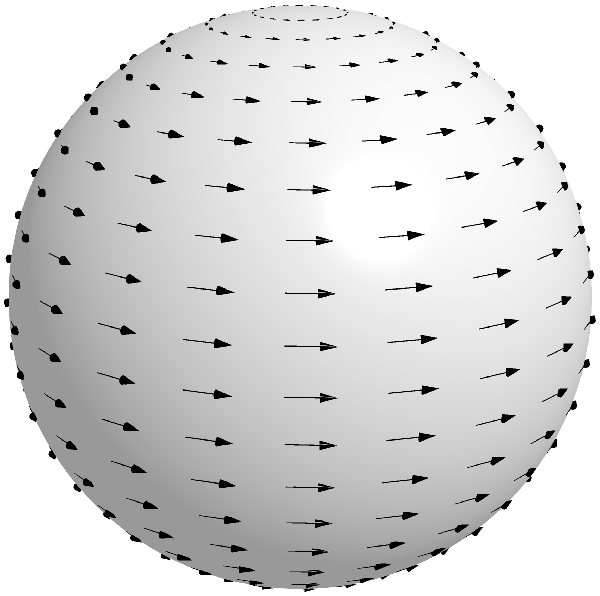
\includegraphics[width=20ex]{figs/sphere_vf_rotate.pdf}

Rotation: index +1 at each pole = \textbf{2}
\end{column}

\begin{column}{0.5\textwidth}
\centering
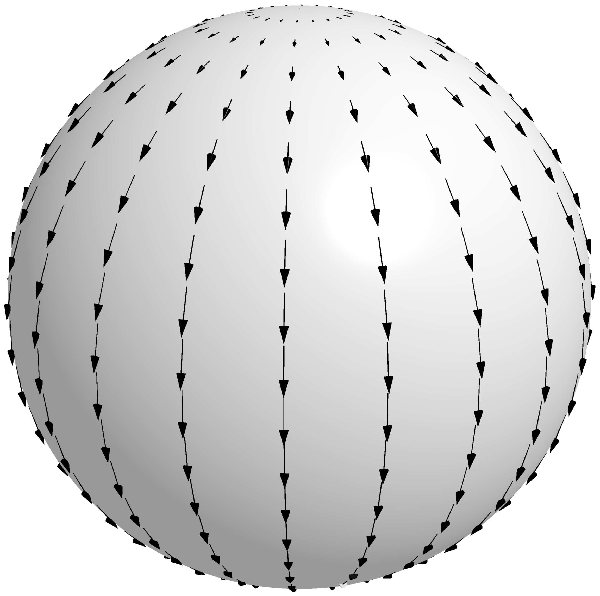
\includegraphics[width=20ex]{figs/sphere_vf_morse.pdf}

Height: index +1 at each pole = \textbf{2}
\end{column}
\end{columns}
\end{frame}

\begin{frame}{Gauss-Bonnet theorem}
Total curvature divided by \( 2\pi \) is the Euler characteristic.

Curvature in 2D is a function \( F_A:M\to \rr \).

\( \int_M F_A \) sums the values at every point. 
\begin{columns}
\begin{column}{0.58\textwidth}
\centering
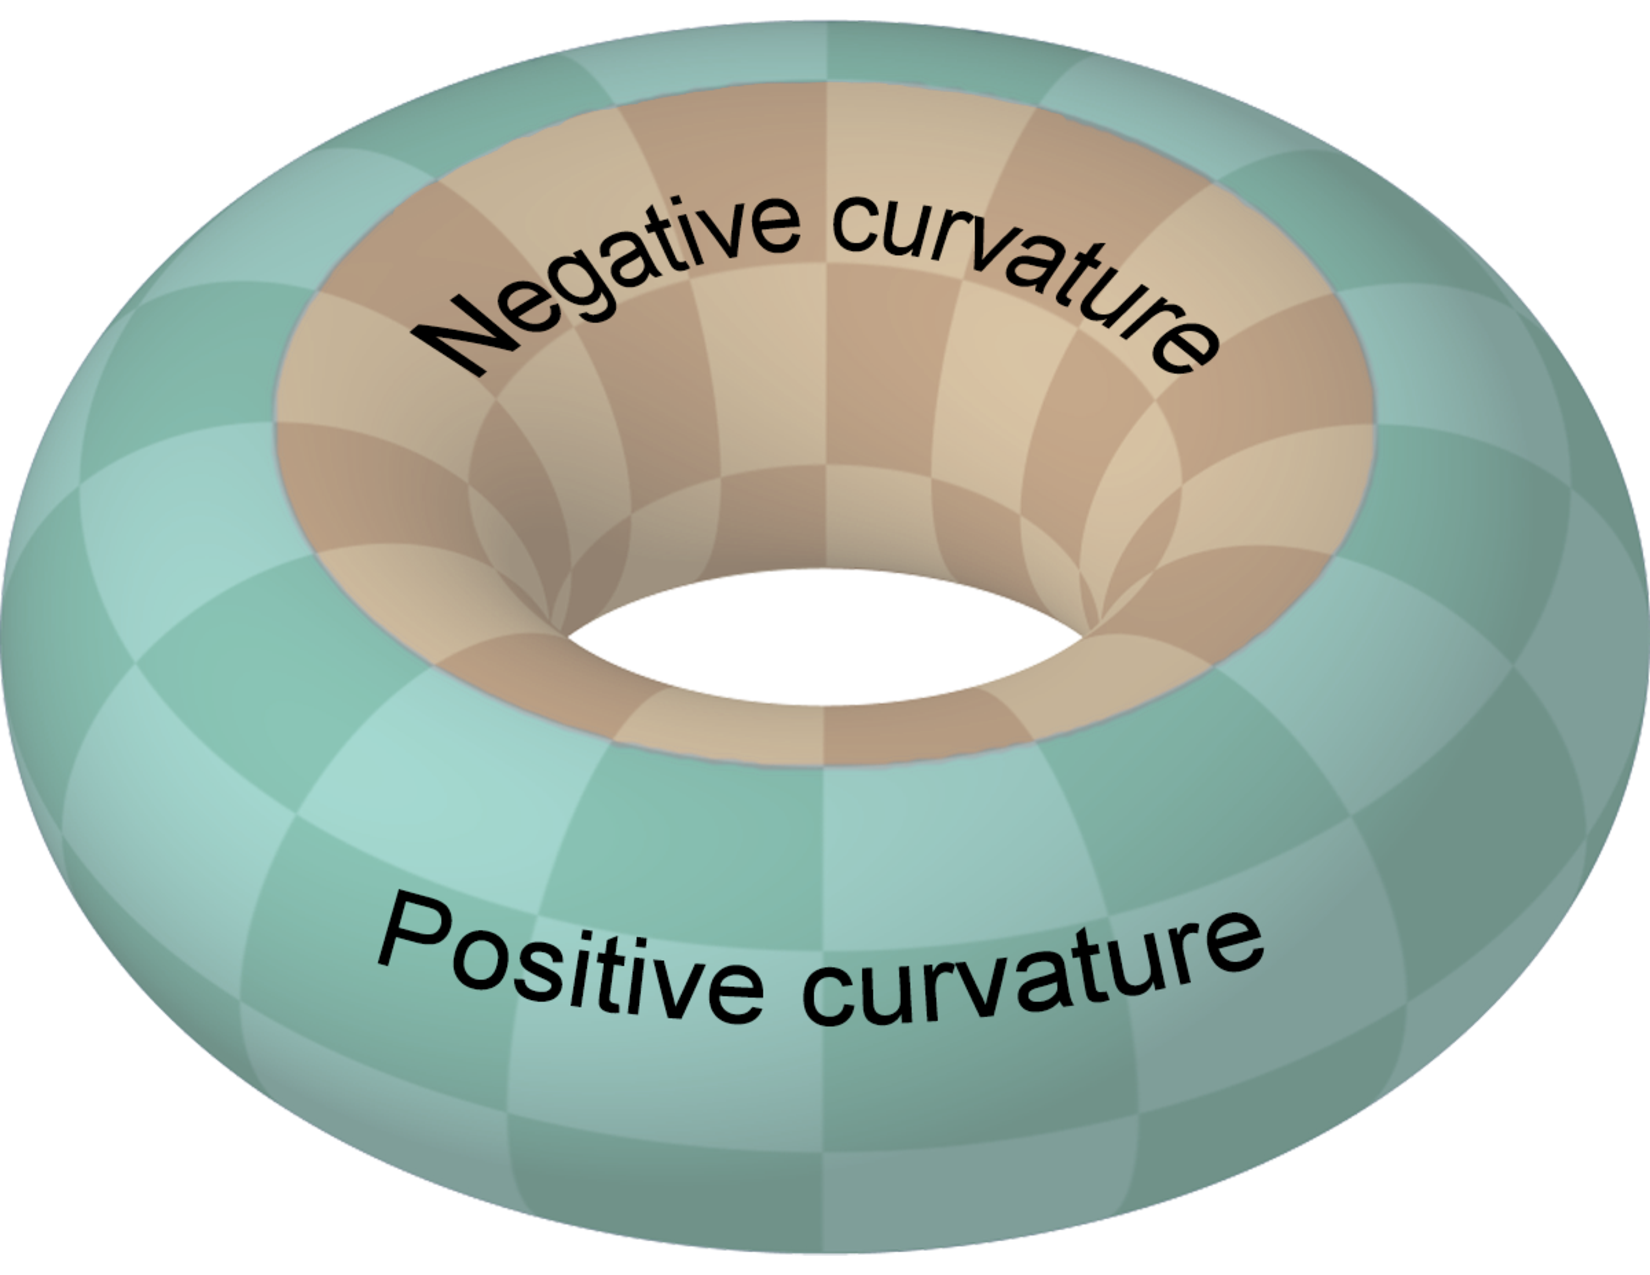
\includegraphics[height=20ex]{figs/torus_gauss_bonnet.pdf}

Positive and negative curvature cancel: \textbf{0}
\end{column}
\begin{column}{0.42\textwidth}
\centering
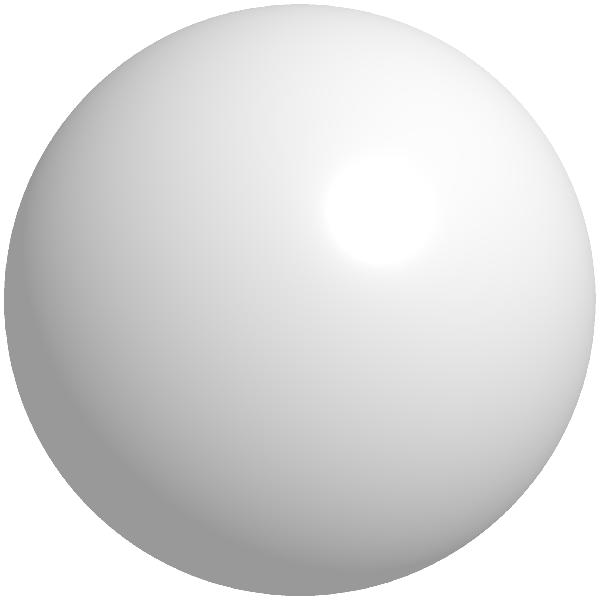
\includegraphics[height=20ex]{figs/sphere_curvature.pdf}

Constant curvature 1, area \( 4\pi \): \textbf{2}
\end{column}
\end{columns}
\end{frame}

\begin{frame}{Plan}
\begin{itemize}
\item Combinatorial manifolds
\item Torsors and classifying maps
\item Connections and curvature
\item Vector fields
\item Main theorem
\end{itemize}
\end{frame}

\begin{frame}{HoTT background}
\begin{enumerate}
\item \alert{Symmetry},\\
Bezem,~M., Buchholtz,~U., Cagne,~P., Dundas,~B.~I., and Grayson,~D.~R., (2021-) \\
\url{https://github.com/UniMath/SymmetryBook}.

\item \alert{Central H-spaces and banded types},\\
Buchholtz,~U., Christensen,~J.~D. , Flaten,~J.~G.~T., and Rijke,~E. (2023) \\
arXiv:2301.02636

\item \alert{Nilpotent types and fracture squares in homotopy type theory},\\
Scoccola,~L. (2020) \\
MSCS 30(5). arXiv:1903.03245
\end{enumerate}
\end{frame}


\section{Combinatorial manifolds}

\begin{frame}{Manifolds in HoTT}
\begin{itemize}
\item Recall the classical theory of \alert{simplicial complexes}
\item Define a \alert{realization} procedure to construct types
\end{itemize}
\end{frame}

\begin{frame}{Simplicial complexes}
\begin{columns}
\begin{column}{0.5\textwidth}
\begin{mydef}
An \defemph{abstract simplicial complex \( M \) of dimension \( n \)} is an ordered list of sets \( M\defeq[M_0,\ldots,M_n] \) consisting of 
\begin{itemize}
\item a set \( M_0 \) of vertices
\item sets \( M_k \) of subsets of \( M_0 \) of cardinality \( k+1 \)
\item downward closed: if \( F\in M_k \) and \( G\subseteq F \), \( |G|=j+1 \) then \( G\in M_j \)
\end{itemize}
We call the truncated list \( M_{\leq k}\defeq [M_0,\ldots,M_k] \) \alert{the \( k \)-skeleton of \( M \)}.
\end{mydef}
\end{column}
\begin{column}{0.5\textwidth}
\resizebox{220pt}{!}{
\onslide<2->{
\begin{tikzpicture}
  \matrix (A) [matrix of math nodes, row sep=1cm, column sep=-.2cm]
  { M_2\\ M_1\\ M_0\\ };
\end{tikzpicture}
\begin{tikzpicture}
    \matrix (A) [matrix of math nodes, row sep=1cm, column sep=-.2cm]
    { 
  ~ &  ~ & \scriptstyle\{w, b, r\} & \scriptstyle\{w, r, g\}  & \scriptstyle\{w, g, o\} & \scriptstyle\{w, o, b\} & \scriptstyle\{y, b, r\} & \scriptstyle\{y, r, g\}  & \scriptstyle\{y, g, o\} & \scriptstyle\{y, o, b\}\\
  \scriptstyle\{w, b\} & \scriptstyle\{w,r\}  & \scriptstyle\{w,g\} & \scriptstyle\{w,o\} & \scriptstyle\{b, r\} & \scriptstyle\{r, g\}  & \scriptstyle\{g, o\} & \scriptstyle\{o, b\} & \scriptstyle\{y, b\} & \scriptstyle\{y,r\}  & \scriptstyle\{y,g\} & \scriptstyle\{y,o\}\\
  ~ & ~ & ~ &  \scriptstyle w  & \scriptstyle b & \scriptstyle r & \scriptstyle g & \scriptstyle o & \scriptstyle y\\
    };

    \draw (A-1-3.south)--(A-2-1.north);
    \draw (A-1-3.south)--(A-2-2.north);
    \draw (A-1-3.south)--(A-2-5.north);

    \draw (A-1-4.south)--(A-2-2.north);
    \draw (A-1-4.south)--(A-2-3.north);
    \draw (A-1-4.south)--(A-2-6.north);

    \draw (A-1-5.south)--(A-2-3.north);
    \draw (A-1-5.south)--(A-2-4.north);
    \draw (A-1-5.south)--(A-2-7.north);

    \draw (A-1-6.south)--(A-2-4.north);
    \draw (A-1-6.south)--(A-2-1.north);
    \draw (A-1-6.south)--(A-2-8.north);

    \draw (A-1-7.south)--(A-2-5.north);
    \draw (A-1-7.south)--(A-2-10.north);
    \draw (A-1-7.south)--(A-2-9.north);

    \draw (A-1-8.south)--(A-2-6.north);
    \draw (A-1-8.south)--(A-2-11.north);
    \draw (A-1-8.south)--(A-2-10.north);

    \draw (A-1-9.south)--(A-2-7.north);
    \draw (A-1-9.south)--(A-2-12.north);
    \draw (A-1-9.south)--(A-2-11.north);

    \draw (A-1-10.south)--(A-2-8.north);
    \draw (A-1-10.south)--(A-2-9.north);
    \draw (A-1-10.south)--(A-2-12.north);

    \draw (A-2-1.south)--(A-3-4.north);
    \draw (A-2-1.south)--(A-3-5.north);

    \draw (A-2-2.south)--(A-3-4.north);
    \draw (A-2-2.south)--(A-3-6.north);

    \draw (A-2-3.south)--(A-3-4.north);
    \draw (A-2-3.south)--(A-3-7.north);

    \draw (A-2-4.south)--(A-3-4.north);
    \draw (A-2-4.south)--(A-3-8.north);

    \draw (A-2-5.south)--(A-3-5.north);
    \draw (A-2-5.south)--(A-3-6.north);

    \draw (A-2-6.south)--(A-3-6.north);
    \draw (A-2-6.south)--(A-3-7.north);

    \draw (A-2-7.south)--(A-3-7.north);
    \draw (A-2-7.south)--(A-3-8.north);

    \draw (A-2-8.south)--(A-3-8.north);
    \draw (A-2-8.south)--(A-3-5.north);

    \draw (A-2-9.south)--(A-3-9.north);
    \draw (A-2-9.south)--(A-3-5.north);

    \draw (A-2-10.south)--(A-3-9.north);
    \draw (A-2-10.south)--(A-3-6.north);

    \draw (A-2-11.south)--(A-3-9.north);
    \draw (A-2-11.south)--(A-3-7.north);

    \draw (A-2-12.south)--(A-3-9.north);
    \draw (A-2-12.south)--(A-3-8.north);
\end{tikzpicture}
}
}
\onslide<2->{\begin{figure}[h]
\centering
\begin{tikzpicture}%
  [x={(-0.860769cm, -0.121512cm)},
  y={(0.508996cm, -0.205391cm)},
  z={(-0.000053cm, 0.971107cm)},
  scale=1,
  back/.style={loosely dotted, thin},
  edge/.style={black, thick},
  facet/.style={fill=blue!95!black,fill opacity=0.1},
  vertex/.style={inner sep=1pt,circle,draw=green!25!black,fill=black,thick}]
\coordinate (-1, -1, 0) at (-1, -1, 0);
\coordinate (-1, 1, 0) at (-1, 1, 0);
\coordinate (0, 0, -1) at (0, 0, -1);
\coordinate (0, 0, 1) at (0, 0, 1);
\coordinate (1, -1, 0) at (1, -1, 0);
\coordinate (1, 1, 0) at (1, 1, 0);
%% Drawing edges in the back
%%
\draw[edge,back] (-1, -1, 0) -- (-1, 1, 0);
\draw[edge,back] (-1, -1, 0) -- (0, 0, -1.4);
\draw[edge,back] (-1, -1, 0) -- (0, 0, 1.4);
\draw[edge,back] (-1, -1, 0) -- (1, -1, 0);
%% Drawing vertices in the back
%%
\node[vertex] at (-1, -1, 0)     {};
%% Drawing the facets
%%
\fill[facet] (1, 1, 0) -- (0, 0, -1.4) -- (1, -1, 0) -- cycle {};
\fill[facet] (1, 1, 0) -- (0, 0, 1.4) -- (1, -1, 0) -- cycle {};
\fill[facet] (1, 1, 0) -- (-1, 1, 0) -- (0, 0, 1.4) -- cycle {};
\fill[facet] (1, 1, 0) -- (-1, 1, 0) -- (0, 0, -1.4) -- cycle {};
%% Drawing edges in the front
%%
\draw[edge] (-1, 1, 0) -- (0, 0, -1.4);
\draw[edge] (-1, 1, 0) -- (0, 0, 1.4);
\draw[edge] (-1, 1, 0) -- (1, 1, 0);
\draw[edge] (0, 0, -1.4) -- (1, -1, 0);
\draw[edge] (0, 0, -1.4) -- (1, 1, 0);
\draw[edge] (0, 0, 1.4) -- (1, -1, 0);
\draw[edge] (0, 0, 1.4) -- (1, 1, 0);
\draw[edge] (1, -1, 0) -- (1, 1, 0);
%% Drawing the vertices in the front
%%
\begin{scope}[nodes=vertex]
\node[label=above right:\( b \)] at (-1, 1, 0)     {};
\node[label=below:\( y \)] at (0, 0, -1.4)     {};
\node[label=above:\( w \)] at (0, 0, 1.4)     {};
\node[label=above left:\( g \)] at (1, -1, 0)     {};
\node[label=above left:\( r \)] at (1, 1, 0)     {};
\node[label=above right:\( o \)] at (-1, -1, 0)     {};
\end{scope}
\end{tikzpicture}
\caption{The HIT \( \oo \) which has 6 points, 12 1-paths, 8 2-paths.}
\end{figure}
}
\onslide<2->{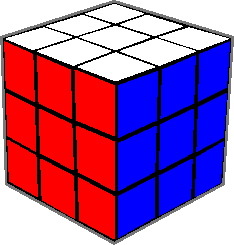
\includegraphics[width=60pt]{figs/hungarian_cube.pdf}}
\end{column}
\end{columns}
\end{frame}

\begin{frame}{Simplicial complexes}
\begin{example}
The \defemph{complete simplex of dimension \( n \)}, denoted \alert{\( \Delta(n), \)} is the set \( \{0,\ldots,n\} \) and its power set. The \( (n-1) \)-skeleton \( \Delta(n)_{\leq (n-1)} \) is denoted \alert{\( \partial \Delta(n) \)} and will serve as a combinatorial \( (n-1) \)-sphere.
\end{example}
\( \Delta(1) \) is visually 
\begin{tikzpicture}[baseline=-1.2mm]
\tikzset{oo/.style={circle, scale=0.25, fill=black}}
\node[oo, label=left:\( 0 \)] at (-0.7, 0) (a) {};
\node[oo, label=right:\( 1 \)] at  (0.7, 0) (c) {};
\draw[fill=blue!95!black,fill opacity=0.1] (-0.7, 0)--(0.7, 0);
\end{tikzpicture}, 
\( \partial\Delta(1) \) is visually
\begin{tikzpicture}[baseline=-1.2mm]
\tikzset{oo/.style={circle, scale=0.25, fill=black}}
\node[oo, label=left:\( 0 \)] at (-0.7, 0) (a) {};
\node[oo, label=right:\( 1 \)] at  (0.7, 0) (c) {};
\end{tikzpicture}, 

\( \Delta(2) \) is visually 
\begin{tikzpicture}[baseline=3mm]
\tikzset{oo/.style={circle, scale=0.25, fill=black}}
\node[oo, label=left:\( 0 \)] at (-0.7, 0) (a) {};
\node[oo, label=right:\( 1 \)] at  (0, 1) (b) {};
\node[oo, label=right:\( 2 \)] at  (0.7, 0) (c) {};
\draw[fill=blue!95!black,fill opacity=0.1] (-0.7, 0)--(0, 1)--(0.7, 0)--(a);
\end{tikzpicture}, 
\( \partial \Delta(2) \) is visually 
\begin{tikzpicture}[baseline=3mm]
\tikzset{oo/.style={circle, scale=0.25, fill=black}}
\node[oo, label=left:\( 0 \)] at (-0.7, 0) (a) {};
\node[oo, label=right:\( 1 \)] at  (0, 1) (b) {};
\node[oo, label=right:\( 2 \)] at  (0.7, 0) (c) {};
\draw (a) -- (b);
\draw (b) -- (c);
\draw (c) -- (a);
\end{tikzpicture}
\end{frame}

\begin{frame}{Homotopy realization: dimension 0}
We will \alert{realize} simplicial complexes by means of \alert{a sequence of pushouts}.

Base case: the realization \( \mm \) of a 0-dimensional complex \( M \) is \( M_0 \).

In particular the 0-sphere \( \partial\Dd(1)\defeq \partial \Delta(1)_0 \).
\end{frame}

\begin{frame}{Homotopy realization: dimension 1}
For a 1-dim complex \( M\defeq [M_0,M_1] \) the realization is given by
\[% https://q.uiver.app/#q=WzAsNCxbMCwxLCJNXzA9XFxtYXRoYmJ7TX1fMCJdLFsxLDEsIlxcbWF0aGJie019XzEiXSxbMSwwLCJNXzEiXSxbMCwwLCJNXzFcXHRpbWVzIFxcYmRzaW1wbGV4bnsxfSJdLFswLDFdLFszLDAsIlxcbWF0aGJie0F9XzAiLDJdLFszLDIsIlxcbWF0aHJte3ByfV8xIl0sWzIsMSwiKl97XFxtYXRoYmJ7TX1fMX0iXSxbMSwzLCIiLDIseyJvZmZzZXQiOjMsInN0eWxlIjp7Im5hbWUiOiJjb3JuZXItaW52ZXJzZSJ9fV0sWzAsMiwiaF8xIiwyLHsic2hvcnRlbiI6eyJzb3VyY2UiOjQwLCJ0YXJnZXQiOjQwfSwibGV2ZWwiOjJ9XV0=
\begin{tikzcd}
  {M_1\times \bdsimplexn{1}} & {M_1} \\
  {M_0=\mathbb{M}_0} & {\mathbb{M}_1}
  \arrow["{\mathrm{pr}_1}", from=1-1, to=1-2]
  \arrow["{\mathbb{A}_0}"', from=1-1, to=2-1]
  \arrow["{*_{\mathbb{M}_1}}", from=1-2, to=2-2]
  \arrow["{h_1}"', shorten <=14pt, shorten >=14pt, Rightarrow, from=2-1, to=1-2]
  \arrow[from=2-1, to=2-2]
  \arrow["\ulcorner"{pos=0, rotate=180}, shift left=1, draw=none, from=2-2, to=1-1]
\end{tikzcd}

\]
\end{frame}

\begin{frame}{Homotopy realization: dimension 1}
For example the simplicial 1-sphere \( \partial\Dd(2)\defeq \)
\begin{tikzpicture}[baseline=3mm, scale=0.7]
\tikzset{oo/.style={circle, scale=0.25, fill=black}}
\node[oo, label=left:\( 0 \)] at (-0.7, 0) (a) {};
\node[oo, label=right:\( 1 \)] at  (0, 1) (b) {};
\node[oo, label=right:\( 2 \)] at  (0.7, 0) (c) {};
\draw (a) -- (b);
\draw (b) -- (c);
\draw (c) -- (a);
\end{tikzpicture} is given by
\vspace{3ex}
\begin{columns}
\begin{column}{0.4\textwidth}
% https://q.uiver.app/#q=WzAsNCxbMSwwLCJcXHBhcnRpYWwgXFxEZWx0YSgyKV8xIl0sWzEsMSwiXFxwYXJ0aWFsXFxEZCgyKSJdLFswLDAsIlxccGFydGlhbCBcXERlbHRhKDIpXzFcXHRpbWVzIFxccGFydGlhbFxcRGQoMSkiXSxbMCwxLCJcXHBhcnRpYWwgXFxEZWx0YSgyKV8wIl0sWzIsMF0sWzIsM10sWzMsMV0sWzAsMV0sWzEsMiwiIiwxLHsic3R5bGUiOnsibmFtZSI6ImNvcm5lci1pbnZlcnNlIn19XSxbMywwLCJoXzEiLDIseyJzaG9ydGVuIjp7InNvdXJjZSI6MzAsInRhcmdldCI6MzB9LCJsZXZlbCI6Mn1dXQ==
\begin{tikzcd}[ampersand replacement=\&]
  {\partial \Delta(2)_1\times \partial\Dd(1)} \& {\partial \Delta(2)_1} \\
  {\partial \Delta(2)_0} \& {\partial\Dd(2)}
  \arrow[from=1-1, to=1-2]
  \arrow[from=1-1, to=2-1]
  \arrow[from=1-2, to=2-2]
  \arrow["{h_1}"', shorten <=11pt, shorten >=11pt, Rightarrow, from=2-1, to=1-2]
  \arrow[from=2-1, to=2-2]
  \arrow["\ulcorner"{pos=0, rotate=180}, draw=none, from=2-2, to=1-1]
\end{tikzcd}
\end{column}
\begin{column}{0.05\textwidth}
i.e.
\end{column}
\begin{column}{0.6\textwidth}
% https://q.uiver.app/#q=WzAsNCxbMSwwLCJcXHNjcmlwdHN0eWxlXFx7XFx7MCwgMVxcfSwgXFx7MSwgMlxcfSwgXFx7MiwgMFxcfVxcfSJdLFsxLDEsIlxccGFydGlhbFxcRGQoMikiXSxbMCwwLCJcXHNjcmlwdHN0eWxlXFx7XFx7MCwgMVxcfSwgXFx7MSwgMlxcfSwgXFx7MiwgMFxcfVxcfVxcdGltZXMgXFx7MCwgMVxcfSJdLFswLDEsIlxcc2NyaXB0c3R5bGVcXHswLCAxLCAyXFx9Il0sWzIsMF0sWzIsM10sWzMsMV0sWzAsMV0sWzEsMiwiIiwxLHsic3R5bGUiOnsibmFtZSI6ImNvcm5lci1pbnZlcnNlIn19XSxbMywwLCJoXzEiLDIseyJzaG9ydGVuIjp7InNvdXJjZSI6MzAsInRhcmdldCI6MzB9LCJsZXZlbCI6Mn1dXQ==
\begin{tikzcd}[ampersand replacement=\&]
  {\scriptstyle\{\{0, 1\}, \{1, 2\}, \{2, 0\}\}\times \{0, 1\}} \& {\scriptstyle\{\{0, 1\}, \{1, 2\}, \{2, 0\}\}} \\
  {\scriptstyle\{0, 1, 2\}} \& {\partial\Dd(2)}
  \arrow[from=1-1, to=1-2]
  \arrow[from=1-1, to=2-1]
  \arrow[from=1-2, to=2-2]
  \arrow["{h_1}"', shorten <=13pt, shorten >=13pt, Rightarrow, from=2-1, to=1-2]
  \arrow[from=2-1, to=2-2]
  \arrow["\ulcorner"{pos=0, rotate=180}, draw=none, from=2-2, to=1-1]
\end{tikzcd}
\end{column}
\end{columns}
\end{frame}

\begin{frame}{Homotopy realization: dimension 1}
Or the 1-skeleton of the octahedron \( \oo \):
% https://q.uiver.app/#q=WzAsNCxbMCwxLCJcXHt3LCBnLFxcbGRvdHNcXH0iXSxbMCwwLCJcXHtcXHt3LCBnXFx9LFxcbGRvdHNcXH1cXHRpbWVzXFx7MCwxXFx9Il0sWzEsMCwiXFx7XFx7dyxnXFx9LFxcbGRvdHNcXH0iXSxbMSwxLCJcXG9vXzEiXSxbMSwyXSxbMSwwXSxbMCwzXSxbMiwzXSxbMywxLCIiLDEseyJzdHlsZSI6eyJuYW1lIjoiY29ybmVyLWludmVyc2UifX1dLFswLDIsImhfMSIsMix7InNob3J0ZW4iOnsic291cmNlIjozMCwidGFyZ2V0IjozMH0sImxldmVsIjoyfV1d
\[\begin{tikzcd}[ampersand replacement=\&]
  {\{\{w, g\},\ldots\}\times\{0,1\}} \& {\{\{w,g\},\ldots\}} \\
  {\{w, g,\ldots\}} \& {\oo_1}
  \arrow[from=1-1, to=1-2]
  \arrow[from=1-1, to=2-1]
  \arrow[from=1-2, to=2-2]
  \arrow["{h_1}"', shorten <=11pt, shorten >=11pt, Rightarrow, from=2-1, to=1-2]
  \arrow[from=2-1, to=2-2]
  \arrow["\ulcorner"{anchor=center, pos=0.125, rotate=180}, draw=none, from=2-2, to=1-1]
\end{tikzcd}\]
\begin{tikzpicture}%
  [x={(-0.860769cm, -0.121512cm)},
  y={(0.508996cm, -0.205391cm)},
  z={(-0.000053cm, 0.971107cm)},
  scale=1,
  back/.style={loosely dotted, thin},
  edge/.style={black, thick},
  facet/.style={fill=blue!95!black,fill opacity=0.0},
  vertex/.style={inner sep=1pt,circle,draw=green!25!black,fill=black,thick}]
\coordinate (-1, -1, 0) at (-1, -1, 0);
\coordinate (-1, 1, 0) at (-1, 1, 0);
\coordinate (0, 0, -1) at (0, 0, -1);
\coordinate (0, 0, 1) at (0, 0, 1);
\coordinate (1, -1, 0) at (1, -1, 0);
\coordinate (1, 1, 0) at (1, 1, 0);
%% Drawing edges in the back
%%
\draw[edge,back] (-1, -1, 0) -- (-1, 1, 0);
\draw[edge,back] (-1, -1, 0) -- (0, 0, -1.4);
\draw[edge,back] (-1, -1, 0) -- (0, 0, 1.4);
\draw[edge,back] (-1, -1, 0) -- (1, -1, 0);
%% Drawing vertices in the back
%%
\node[vertex] at (-1, -1, 0)     {};
%% Drawing the facets
%%
\fill[facet] (1, 1, 0) -- (0, 0, -1.4) -- (1, -1, 0) -- cycle {};
\fill[facet] (1, 1, 0) -- (0, 0, 1.4) -- (1, -1, 0) -- cycle {};
\fill[facet] (1, 1, 0) -- (-1, 1, 0) -- (0, 0, 1.4) -- cycle {};
\fill[facet] (1, 1, 0) -- (-1, 1, 0) -- (0, 0, -1.4) -- cycle {};
%% Drawing edges in the front
%%
\draw[edge] (-1, 1, 0) -- (0, 0, -1.4);
\draw[edge] (-1, 1, 0) -- (0, 0, 1.4);
\draw[edge] (-1, 1, 0) -- (1, 1, 0);
\draw[edge] (0, 0, -1.4) -- (1, -1, 0);
\draw[edge] (0, 0, -1.4) -- (1, 1, 0);
\draw[edge] (0, 0, 1.4) -- (1, -1, 0);
\draw[edge] (0, 0, 1.4) -- (1, 1, 0);
\draw[edge] (1, -1, 0) -- (1, 1, 0);
%% Drawing the vertices in the front
%%
\begin{scope}[nodes=vertex]
\node[label=above right:\( b \)] at (-1, 1, 0)     {};
\node[label=below:\( y \)] at (0, 0, -1.4)     {};
\node[label=above:\( w \)] at (0, 0, 1.4)     {};
\node[label=above left:\( g \)] at (1, -1, 0)     {};
\node[label=above left:\( r \)] at (1, 1, 0)     {};
\node[label=above right:\( o \)] at (-1, -1, 0)     {};
\end{scope}
\end{tikzpicture}

\end{frame}

\begin{frame}{Homotopy realization: dimension 2}
To realize \( M\defeq[M_0, M_1, M_2] \) use \(  \partial\Dd(1), \partial\Dd(2) \):
\[% https://q.uiver.app/#q=WzAsNyxbMCwwLCJNXzFcXHRpbWVzIFxccGFydGlhbFxcRGQoMSkiXSxbMCwxLCJNXzA9XFxtYXRoYmJ7TX1fMCJdLFsxLDEsIlxcbWF0aGJie019XzEiXSxbMSwwLCJNXzEiXSxbMSwyLCJNXzJcXHRpbWVzIFxccGFydGlhbFxcRGQoMikiXSxbMiwyLCJNXzIiXSxbMiwxLCJcXG1hdGhiYntNfV8yIl0sWzAsMSwiXFxtYXRoYmJ7QX1fMCIsMl0sWzEsMl0sWzAsMywiXFxtYXRocm17cHJ9XzEiXSxbMywyLCIqX3tcXG1hdGhiYntNfV8xfSJdLFsyLDAsIiIsMSx7InN0eWxlIjp7Im5hbWUiOiJjb3JuZXItaW52ZXJzZSJ9fV0sWzIsNl0sWzQsMiwiXFxtYXRoYmJ7QX1fMSJdLFs1LDYsIipfe1xcbWF0aGJie019XzJ9IiwyXSxbNCw1LCJcXG1hdGhybXtwcn1fMSIsMl0sWzYsNCwiIiwxLHsic3R5bGUiOnsibmFtZSI6ImNvcm5lci1pbnZlcnNlIn19XSxbMiw1LCJoXzIiLDAseyJzaG9ydGVuIjp7InNvdXJjZSI6NDAsInRhcmdldCI6NDB9LCJsZXZlbCI6Mn1dLFsxLDMsImhfMSIsMix7InNob3J0ZW4iOnsic291cmNlIjo0MCwidGFyZ2V0Ijo0MH0sImxldmVsIjoyfV1d
\begin{tikzcd}[ampersand replacement=\&]
  {M_1\times \partial\Dd(1)} \& {M_1} \\
  {M_0=\mathbb{M}_0} \& {\mathbb{M}_1} \& {\mathbb{M}_2} \\
  \& {M_2\times \partial\Dd(2)} \& {M_2}
  \arrow["{\mathrm{pr}_1}", from=1-1, to=1-2]
  \arrow["{\mathbb{A}_0}"', from=1-1, to=2-1]
  \arrow["{*_{\mathbb{M}_1}}", from=1-2, to=2-2]
  \arrow["{h_1}"', shorten <=17pt, shorten >=17pt, Rightarrow, from=2-1, to=1-2]
  \arrow[from=2-1, to=2-2]
  \arrow["\ulcorner"{anchor=center, pos=0.125, rotate=180}, draw=none, from=2-2, to=1-1]
  \arrow[from=2-2, to=2-3]
  \arrow["{h_2}", shorten <=13pt, shorten >=13pt, Rightarrow, from=2-2, to=3-3]
  \arrow["\ulcorner"{anchor=center, pos=0.125, rotate=-90}, draw=none, from=2-3, to=3-2]
  \arrow["{\mathbb{A}_1}", from=3-2, to=2-2]
  \arrow["{\mathrm{pr}_1}"', from=3-2, to=3-3]
  \arrow["{*_{\mathbb{M}_2}}"', from=3-3, to=2-3]
\end{tikzcd}
\]
\end{frame}

\begin{frame}{Homotopy realization: dimension 2}
The full octahedron \( \oo \):
\begin{columns}
\begin{column}{0.75\textwidth}
% https://q.uiver.app/#q=WzAsNyxbMCwwLCJcXHtcXHt3LCBnXFx9LFxcbGRvdHNcXH1cXHRpbWVzXFx7MCwxXFx9Il0sWzAsMSwiXFx7dywgZyxcXGxkb3RzXFx9Il0sWzEsMSwiXFxvb18xIl0sWzEsMCwiXFx7XFx7dyxnXFx9LFxcbGRvdHNcXH0iXSxbMSwyLCJcXHtcXHt3LGcsclxcfSxcXGxkb3RzXFx9XFx0aW1lcyBcXHBhcnRpYWxcXERkKDIpIl0sWzIsMiwiXFx7XFx7dyxnLHJcXH0sXFxsZG90c1xcfSJdLFsyLDEsIlxcb29fMiJdLFswLDFdLFsxLDJdLFswLDMsIlxcbWF0aHJte3ByfV8xIl0sWzMsMl0sWzIsMCwiIiwxLHsic3R5bGUiOnsibmFtZSI6ImNvcm5lci1pbnZlcnNlIn19XSxbMiw2XSxbNCwyXSxbNSw2XSxbNCw1LCJcXG1hdGhybXtwcn1fMSIsMl0sWzYsNCwiIiwxLHsic3R5bGUiOnsibmFtZSI6ImNvcm5lci1pbnZlcnNlIn19XSxbMiw1LCJoXzIiLDAseyJzaG9ydGVuIjp7InNvdXJjZSI6NDAsInRhcmdldCI6NDB9LCJsZXZlbCI6Mn1dLFsxLDMsImhfMSIsMix7InNob3J0ZW4iOnsic291cmNlIjo0MCwidGFyZ2V0Ijo0MH0sImxldmVsIjoyfV1d
\[\begin{tikzcd}[ampersand replacement=\&, column sep=small]
  {\{\{w, g\},\ldots\}\times\{0,1\}} \& {\{\{w,g\},\ldots\}} \\
  {\{w, g,\ldots\}} \& {\oo_1} \& {\oo_2} \\
  \& {\{\{w,g,r\},\ldots\}\times \partial\Dd(2)} \& {\{\{w,g,r\},\ldots\}}
  \arrow["{\mathrm{pr}_1}", from=1-1, to=1-2]
  \arrow[from=1-1, to=2-1]
  \arrow[from=1-2, to=2-2]
  \arrow["{h_1}"', shorten <=22pt, shorten >=22pt, Rightarrow, from=2-1, to=1-2]
  \arrow[from=2-1, to=2-2]
  \arrow["\ulcorner"{pos=0.05, rotate=180}, draw=none, from=2-2, to=1-1]
  \arrow[from=2-2, to=2-3]
  \arrow["{h_2}", shorten <=21pt, shorten >=21pt, Rightarrow, from=2-2, to=3-3]
  \arrow["\ulcorner"{pos=-0.1, rotate=-90}, draw=none, from=2-3, to=3-2]
  \arrow[from=3-2, to=2-2]
  \arrow["{\mathrm{pr}_1}"', from=3-2, to=3-3]
  \arrow[from=3-3, to=2-3]
\end{tikzcd}\]
\end{column}
\begin{column}{0.25\textwidth}
\begin{figure}[h]
\centering
\begin{tikzpicture}%
  [x={(-0.860769cm, -0.121512cm)},
  y={(0.508996cm, -0.205391cm)},
  z={(-0.000053cm, 0.971107cm)},
  scale=1,
  back/.style={loosely dotted, thin},
  edge/.style={black, thick},
  facet/.style={fill=blue!95!black,fill opacity=0.1},
  vertex/.style={inner sep=1pt,circle,draw=green!25!black,fill=black,thick}]
\coordinate (-1, -1, 0) at (-1, -1, 0);
\coordinate (-1, 1, 0) at (-1, 1, 0);
\coordinate (0, 0, -1) at (0, 0, -1);
\coordinate (0, 0, 1) at (0, 0, 1);
\coordinate (1, -1, 0) at (1, -1, 0);
\coordinate (1, 1, 0) at (1, 1, 0);
%% Drawing edges in the back
%%
\draw[edge,back] (-1, -1, 0) -- (-1, 1, 0);
\draw[edge,back] (-1, -1, 0) -- (0, 0, -1.4);
\draw[edge,back] (-1, -1, 0) -- (0, 0, 1.4);
\draw[edge,back] (-1, -1, 0) -- (1, -1, 0);
%% Drawing vertices in the back
%%
\node[vertex] at (-1, -1, 0)     {};
%% Drawing the facets
%%
\fill[facet] (1, 1, 0) -- (0, 0, -1.4) -- (1, -1, 0) -- cycle {};
\fill[facet] (1, 1, 0) -- (0, 0, 1.4) -- (1, -1, 0) -- cycle {};
\fill[facet] (1, 1, 0) -- (-1, 1, 0) -- (0, 0, 1.4) -- cycle {};
\fill[facet] (1, 1, 0) -- (-1, 1, 0) -- (0, 0, -1.4) -- cycle {};
%% Drawing edges in the front
%%
\draw[edge] (-1, 1, 0) -- (0, 0, -1.4);
\draw[edge] (-1, 1, 0) -- (0, 0, 1.4);
\draw[edge] (-1, 1, 0) -- (1, 1, 0);
\draw[edge] (0, 0, -1.4) -- (1, -1, 0);
\draw[edge] (0, 0, -1.4) -- (1, 1, 0);
\draw[edge] (0, 0, 1.4) -- (1, -1, 0);
\draw[edge] (0, 0, 1.4) -- (1, 1, 0);
\draw[edge] (1, -1, 0) -- (1, 1, 0);
%% Drawing the vertices in the front
%%
\begin{scope}[nodes=vertex]
\node[label=above right:\( b \)] at (-1, 1, 0)     {};
\node[label=below:\( y \)] at (0, 0, -1.4)     {};
\node[label=above:\( w \)] at (0, 0, 1.4)     {};
\node[label=above left:\( g \)] at (1, -1, 0)     {};
\node[label=above left:\( r \)] at (1, 1, 0)     {};
\node[label=above right:\( o \)] at (-1, -1, 0)     {};
\end{scope}
\end{tikzpicture}
\caption{The HIT \( \oo \) which has 6 points, 12 1-paths, 8 2-paths.}
\end{figure}

\end{column}
\end{columns}
\end{frame}

\begin{frame}{Homotopy realization: dimension 2}
\begin{columns}
\begin{column}{0.25\textwidth}
\begin{tikzpicture}%
  [x={(-0.860769cm, -0.121512cm)},
  y={(0.508996cm, -0.205391cm)},
  z={(-0.000053cm, 0.971107cm)},
  scale=1,
  eqback/.style={very thick},
  back/.style={loosely dotted, thin},
  eqedge/.style={very thick},
  edge/.style={black, thin},
  r/.style={},
  facet/.style={fill=blue!95!black,fill opacity=0.0},
  vertex/.style={inner sep=1pt,circle,draw=green!25!black,fill=black,thick}]
\coordinate (-1, -1, 0) at (-1, -1, 0);
\coordinate (-1, 1, 0) at (-1, 1, 0);
\coordinate (0, 0, -1) at (0, 0, -1);
\coordinate (0, 0, 1) at (0, 0, 1);
\coordinate (1, -1, 0) at (1, -1, 0);
\coordinate (1, 1, 0) at (1, 1, 0);
%% Drawing edges in the back
%%
\draw[edge,eqback] (-1, -1, 0) -- (-1, 1, 0);
\draw[edge,back] (-1, -1, 0) -- (0, 0, -1.4);
\draw[edge,back] (-1, -1, 0) -- (0, 0, 1.4);
\draw[edge,eqback] (1, -1, 0) -- (-1, -1, 0);
%% Drawing vertices in the back
%%
\node[vertex] at (-1, -1, 0)     {};
%% Drawing the facets
%%
%\fill[facet] (1, 1, 0) -- (0, 0, -1.4) -- (1, -1, 0) -- cycle {};
%\fill[facet] (1, 1, 0) -- (0, 0, 1.4) -- (1, -1, 0) -- cycle {};
\fill[facet] (1, 1, 0) -- (-1, 1, 0) -- (0, 0, 1.4) -- cycle {};
%\fill[facet] (1, 1, 0) -- (-1, 1, 0) -- (0, 0, -1.4) -- cycle {};
%% Drawing edges in the front
%%
\draw[edge] (-1, 1, 0) -- (0, 0, -1.4);
\draw[edge] (-1, 1, 0) -- (0, 0, 1.4);
\draw[eqedge] (-1, 1, 0) -- (1, 1, 0);
\draw[edge] (0, 0, -1.4) -- (1, -1, 0);
\draw[edge] (0, 0, -1.4) -- (1, 1, 0);
\draw[edge] (0, 0, 1.4) -- (1, -1, 0);
\draw[edge] (0, 0, 1.4) -- (1, 1, 0);
\draw[r,eqedge] (1, 1, 0) -- (1, -1, 0);
%% Drawing the vertices in the front
%%
\begin{scope}[nodes=vertex]
\node[label=above right:\( b \)] at (-1, 1, 0)     {};
\node[label=below:\( y \)] at (0, 0, -1.4)     {};
\node[label=above:\( w \)] at (0, 0, 1.4)     {};
\node[label=above left:\( g \)] at (1, -1, 0)     {};
\node[label=above left:\( r \)] at (1, 1, 0)     {};
\node[label=above right:\( o \)] at (-1, -1, 0)     {};
\end{scope}
\end{tikzpicture}

\end{column}
\begin{column}{0.15\textwidth}
\( \leftarrow\link(w) \)
\end{column}
\begin{column}{0.6\textwidth}
The \defemph{link} of a vertex \( w \) in a 2-complex is: the sets not containing \( w \) but whose union with \( w \) is a face.\\~\\

A \alert{combinatorial manifold} is a simplicial complex all of whose links are\( ^* \) simplicial spheres.\\~\\

This will be our model of the \alert{tangent space}.\\~\\
\end{column}
\end{columns}
\vspace{5ex}
{\scriptsize\( {}^* \)the (classical) geometric realization is homeomorphic to a sphere}
\end{frame}

\begin{frame}{Combinatorial manifolds \( \leftrightarrow \) smooth manifolds}
\begin{theorem}[Whitehead (1940)]
Every smooth \( n \)-manifold has a compatible structure of a \alert{combinatorial manifold}: a simplicial complex of dimension \( n \) such that the link is a combinatorial \( (n-1) \)-sphere, i.e. its geometric realization is an \( (n-1) \)-sphere.
\end{theorem}
\url{https://ncatlab.org/nlab/show/triangulation+theorem}

\onslide<2->{Counterexample: Wikipedia says this is a simplicial complex, but we can see it fails the link condition:

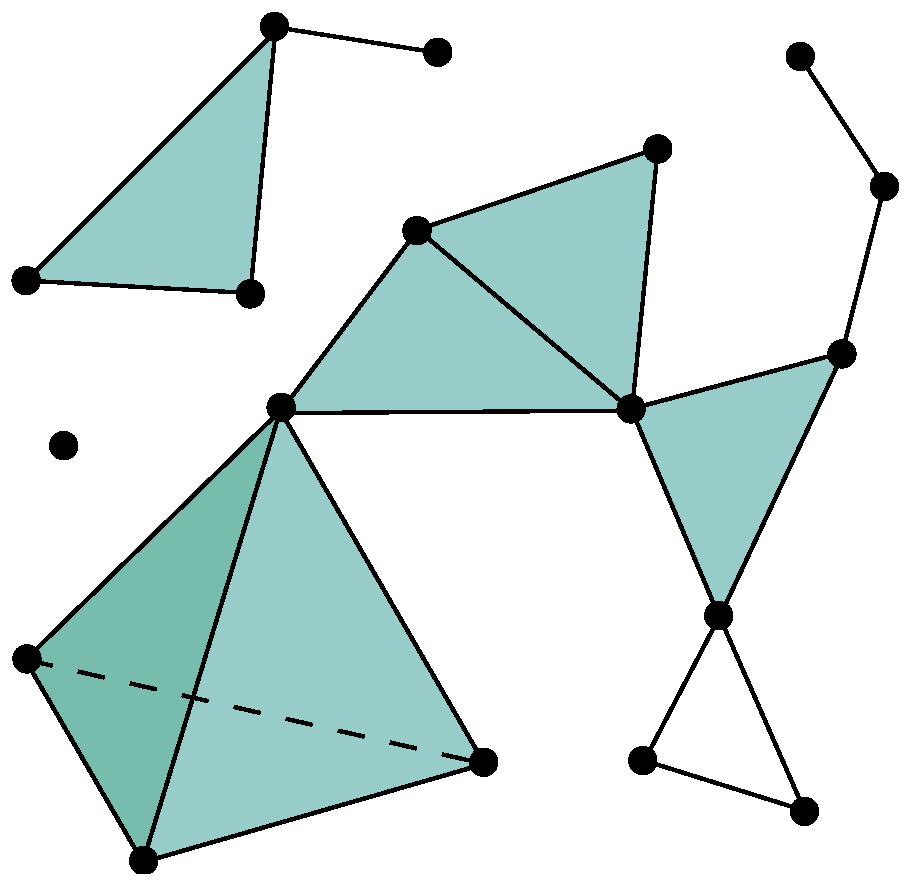
\includegraphics[width=15ex]{figs/simplicial_complex_example.pdf}}
\end{frame}


\section{Torsors}

\begin{frame}
What type families \( \mm\to\uni \) will we consider? Families of \alert{torsors}, also called \alert{principal bundles}.
\end{frame}

\begin{frame}{Torsors}
Let \( G \) be a (higher) group.
\onslide<2->{\begin{definition}
\begin{itemize}
\item<2-> A \defemph{right \( G \)-object} is a type \( X \) equipped with a homomorphism \( \phi:G^{\mathrm{op}}\to\Aut(X) \).
\item<3-> \( X \) is furthermore a \alert{\( G \)-torsor} if it is inhabited and the map \( (\pr_1, \phi):X\times G\to X\times X \) is an equivalence.
\item<4-> The inverse is \( (\pr_1, s) \) where \( s:X\times X\to G \) is called \alert{subtraction} (when \( G \) is commutative).
\item<5-> Let \alert{\( BG \)} be the type of \( G \)-torsors.
\item<6-> Let \( \reg{G} \) be the \( G \)-torsor consisting of \( G \) acting on itself on the right.
\end{itemize}
\end{definition}}
\end{frame}

\begin{frame}{Facts}
\begin{enumerate}
\item<2-> \( \loopy(BG,\reg{G}) \simeq G \) and composition of loops corresponds to multiplication in \( G \).
\item<3-> \( BG \) is connected.
\item<4-> 1 \& 2 \( \implies \) \( BG \) is a \( \K(G,1) \).
\end{enumerate}
\onslide<5->{See the Buchholtz et. al. H-spaces paper for more.}
\end{frame}

\begin{frame}{How to map into \( BS^1 \)}
To construct maps into \( BS^1 \) we \alert{lift} a family of \alert{mere circles}.
% https://q.uiver.app/#q=WzAsNSxbMSwwLCJCU14xIl0sWzIsMCwiXFxCQXV0IChTXjEpXFxzdGFja3JlbHtcXG1hdGhybXtkZWZ9fXs9fVxcc3VtX3tZOlxcdW5pfXx8WT1TXjF8fF97LTF9Il0sWzMsMCwiXFx1bmkiXSxbMiwyLCJcXG1tIl0sWzAsMSwiXFx0ZXh0e2ZhbWlsaWVzIG9mOn0iXSxbMywwLCJcXG1hdGhybXt0b3Jzb3JzfSJdLFszLDEsIlxcc3Vic3RhY2t7XFxtYXRocm17bWVyZX1cXFxcIFxcbWF0aHJte2NpcmNsZXN9fSIsMV0sWzMsMiwiXFxtYXRocm17dHlwZXN9IiwyXSxbMCwxXSxbMSwyXV0=
\[\begin{tikzcd}[ampersand replacement=\&, row sep=small]
  \& {BS^1} \& {\alert{\BAut (S^1)}\stackrel{\mathrm{def}}{=}\sum_{Y:\uni}||Y=S^1||_{-1}} \& \uni \\
  {\text{families of:}} \\
  \&\& \mm
  \arrow[from=1-2, to=1-3]
  \arrow[from=1-3, to=1-4]
  \arrow["{\mathrm{torsors}}", from=3-3, to=1-2]
  \arrow["\begin{array}{c} \substack{\mathrm{mere}\\ \mathrm{circles}} \end{array}"{description}, from=3-3, to=1-3]
  \arrow["{\mathrm{types}}"', from=3-3, to=1-4]
\end{tikzcd}\]
We will assume we have such a lift when we need it. (Remark: the lift is a choice of \alert{orientation}.)

\onslide<2->{
Other names:
\begin{itemize}
\item \( \BAut (S^1)=BO(2)=\EMzo \) (where \( \EM(G,n)\defeq \BAut(\K(G,n)) \))
\item \( BS^1=BSO(2)=\Kzt \)
\end{itemize}}
\end{frame}

% \begin{frame}{A connected component of \( \uni \)?}
% \begin{definition}
% The \alert{type of Eilenberg-Mac Lane spaces \( \EM(G,n) \)} is the connected component of \( \K(G,n) \):
% \[ \EM(G,n)\defeq \BAut(\K(G,n))\defeq \sit{Y:\uni}||Y\simeq \K(G,n)||_{-1} \]
% \end{definition}
% It is a property of a map \( f:A\to\EM(G,n) \) to factor through \( \K(G,n+1) \). See the Scoccola paper.
% \end{frame}

% \begin{frame}{Coincidences of 2 dimensions}
% \begin{itemize}
% \item \( S^1 \) is a \( \Kzo \) since \( \loopy(S^1, \base)\simeq \zz \).
% \item So \( \EMzo \) is a type of \alert{mere circles}.
% \item But \( S^1=_{\EMzo}S^1 \) contains an order 2 \alert{flip}, so \( \not\simeq S^1 \).
% \item For a map \( f:A\to\EMzo \) to factor through  \( \Kzt \), it must somehow avoid flips.
% \item This deserves to be called \alert{orientability}.
% \item \( \link:\mm_0\to\EMzo \) is a great starting point.
% \end{itemize}
% \end{frame}
% 


\section{Connections and curvature}

\begin{frame}{Connections}
Connections are extensions of the bundle to higher skeleta.
\end{frame}

\begin{frame}{Recall \( \link \)}
\begin{columns}
\begin{column}{0.25\textwidth}
\begin{tikzpicture}%
  [x={(-0.860769cm, -0.121512cm)},
  y={(0.508996cm, -0.205391cm)},
  z={(-0.000053cm, 0.971107cm)},
  scale=1,
  eqback/.style={very thick},
  back/.style={loosely dotted, thin},
  eqedge/.style={very thick},
  edge/.style={black, thin},
  r/.style={},
  facet/.style={fill=blue!95!black,fill opacity=0.0},
  vertex/.style={inner sep=1pt,circle,draw=green!25!black,fill=black,thick}]
\coordinate (-1, -1, 0) at (-1, -1, 0);
\coordinate (-1, 1, 0) at (-1, 1, 0);
\coordinate (0, 0, -1) at (0, 0, -1);
\coordinate (0, 0, 1) at (0, 0, 1);
\coordinate (1, -1, 0) at (1, -1, 0);
\coordinate (1, 1, 0) at (1, 1, 0);
%% Drawing edges in the back
%%
\draw[edge,eqback] (-1, -1, 0) -- (-1, 1, 0);
\draw[edge,back] (-1, -1, 0) -- (0, 0, -1.4);
\draw[edge,back] (-1, -1, 0) -- (0, 0, 1.4);
\draw[edge,eqback] (1, -1, 0) -- (-1, -1, 0);
%% Drawing vertices in the back
%%
\node[vertex] at (-1, -1, 0)     {};
%% Drawing the facets
%%
%\fill[facet] (1, 1, 0) -- (0, 0, -1.4) -- (1, -1, 0) -- cycle {};
%\fill[facet] (1, 1, 0) -- (0, 0, 1.4) -- (1, -1, 0) -- cycle {};
\fill[facet] (1, 1, 0) -- (-1, 1, 0) -- (0, 0, 1.4) -- cycle {};
%\fill[facet] (1, 1, 0) -- (-1, 1, 0) -- (0, 0, -1.4) -- cycle {};
%% Drawing edges in the front
%%
\draw[edge] (-1, 1, 0) -- (0, 0, -1.4);
\draw[edge] (-1, 1, 0) -- (0, 0, 1.4);
\draw[eqedge] (-1, 1, 0) -- (1, 1, 0);
\draw[edge] (0, 0, -1.4) -- (1, -1, 0);
\draw[edge] (0, 0, -1.4) -- (1, 1, 0);
\draw[edge] (0, 0, 1.4) -- (1, -1, 0);
\draw[edge] (0, 0, 1.4) -- (1, 1, 0);
\draw[r,eqedge] (1, 1, 0) -- (1, -1, 0);
%% Drawing the vertices in the front
%%
\begin{scope}[nodes=vertex]
\node[label=above right:\( b \)] at (-1, 1, 0)     {};
\node[label=below:\( y \)] at (0, 0, -1.4)     {};
\node[label=above:\( w \)] at (0, 0, 1.4)     {};
\node[label=above left:\( g \)] at (1, -1, 0)     {};
\node[label=above left:\( r \)] at (1, 1, 0)     {};
\node[label=above right:\( o \)] at (-1, -1, 0)     {};
\end{scope}
\end{tikzpicture}

\end{column}
\begin{column}{0.15\textwidth}
\( \leftarrow\link(w) \)
\end{column}
\begin{column}{0.6\textwidth}
The \defemph{link} of a vertex \( w \) in a 2-complex is: the sets not containing \( w \) but whose union with \( w \) is a face.\\~\\
\end{column}
\end{columns}
\end{frame}

\begin{frame}{Connections on the tangent bundle}
An extension \( T_1 \) of \( \link \) to \( \mm_1 \) is called \alert{a connection on the tangent bundle}.
% https://q.uiver.app/#q=WzAsNCxbMSwxLCJcXEJBdXQoU14xKSJdLFswLDAsIlxcbW1fMCJdLFsxLDAsIlxcbW1fMSJdLFsyLDAsIlxcbW1fMiJdLFsxLDAsIlxcbGluayIsMl0sWzIsMCwiVF8xIiwwLHsic3R5bGUiOnsiYm9keSI6eyJuYW1lIjoiZGFzaGVkIn19fV0sWzMsMCwiIiwwLHsic3R5bGUiOnsiYm9keSI6eyJuYW1lIjoiZGFzaGVkIn19fV0sWzEsMl0sWzIsM11d
\[\begin{tikzcd}[ampersand replacement=\&]
  {\mm_0} \& {\mm_1} \& {\mm_2} \\
  \& {\BAut(S^1)}
  \arrow[from=1-1, to=1-2]
  \arrow["\link"', from=1-1, to=2-2]
  \arrow[from=1-2, to=1-3]
  \arrow["{T_1}", dashed, from=1-2, to=2-2]
  \arrow[dashed, from=1-3, to=2-2]
\end{tikzcd}\]
\end{frame}

\begin{frame}{\( T_1:\mm_1\to\BAut(S^1) \) extending \( \link \)}
We will define \( T_1 \) on the edge \( wb \), so we need a term \( T_1(wb):\link(w)=_{\BAut(S^1)}\link(b) \).

We imagine tipping:
\tikzset{every picture/.style={scale=0.85}}
\[\begin{tikzpicture}%
  [x={(-0.860769cm, -0.121512cm)},
  y={(0.508996cm, -0.205391cm)},
  z={(-0.000053cm, 0.971107cm)},
  scale=1,
  eqback/.style={very thick},
  back/.style={loosely dotted, thin},
  eqedge/.style={very thick},
  edge/.style={black, thin},
  r/.style={red},
  facet/.style={fill=blue!95!black,fill opacity=0.0},
  vertex/.style={inner sep=1pt,circle,draw=green!25!black,fill=black,thick},
  baseline=0ex]
\coordinate (-1, -1, 0) at (-1, -1, 0);
\coordinate (-1, 1, 0) at (-1, 1, 0);
\coordinate (0, 0, -1) at (0, 0, -1);
\coordinate (0, 0, 1) at (0, 0, 1);
\coordinate (1, -1, 0) at (1, -1, 0);
\coordinate (1, 1, 0) at (1, 1, 0);
%% Drawing edges in the back
%%
\draw[edge,eqback] (-1, -1, 0) -- (-1, 1, 0);
\draw[edge,back] (-1, -1, 0) -- (0, 0, -1.4);
\draw[edge,back] (-1, -1, 0) -- (0, 0, 1.4);
\draw[edge,eqback] (1, -1, 0) -- (-1, -1, 0);
%% Drawing vertices in the back
%%
\node[vertex] at (-1, -1, 0)     {};
%% Drawing the facets
%%
%\fill[facet] (1, 1, 0) -- (0, 0, -1.4) -- (1, -1, 0) -- cycle {};
%\fill[facet] (1, 1, 0) -- (0, 0, 1.4) -- (1, -1, 0) -- cycle {};
\fill[facet] (1, 1, 0) -- (-1, 1, 0) -- (0, 0, 1.4) -- cycle {};
%\fill[facet] (1, 1, 0) -- (-1, 1, 0) -- (0, 0, -1.4) -- cycle {};
%% Drawing edges in the front
%%
\draw[edge] (-1, 1, 0) -- (0, 0, -1.4);
\draw[edge] (-1, 1, 0) -- (0, 0, 1.4);
\draw[eqedge] (-1, 1, 0) -- (1, 1, 0);
\draw[edge] (0, 0, -1.4) -- (1, -1, 0);
\draw[edge] (0, 0, -1.4) -- (1, 1, 0);
\draw[edge] (0, 0, 1.4) -- (1, -1, 0);
\draw[edge] (0, 0, 1.4) -- (1, 1, 0);
\draw[r,eqedge] (1, 1, 0) -- (1, -1, 0);
%% Drawing the vertices in the front
%%
\begin{scope}[nodes=vertex]
\node[label=above right:\( b \)] at (-1, 1, 0)     {};
\node[label=below:\( y \)] at (0, 0, -1.4)     {};
\node[label=above:\( w \)] at (0, 0, 1.4)     {};
\node[label=above left:\( g \)] at (1, -1, 0)     {};
\node[label=above left:\( r \)] at (1, 1, 0)     {};
\node[label=above right:\( o \)] at (-1, -1, 0)     {};
\end{scope}
\end{tikzpicture}
\quad\longrightarrow\quad \begin{tikzpicture}%
  [x={(-0.860769cm, -0.121512cm)},
  y={(0.508996cm, -0.205391cm)},
  z={(-0.000053cm, 0.971107cm)},
  scale=1,
  eqback/.style={very thick},
  back/.style={loosely dotted, thin},
  eqedge/.style={very thick},
  r/.style={red},
  edge/.style={black, thin},
  facet/.style={fill=blue!95!black,fill opacity=0.0},
  vertex/.style={inner sep=1pt,circle,draw=green!25!black,fill=black,thick},
  baseline=0ex]
\coordinate (-1, -1, 0) at (-1, -1, 0);
\coordinate (-1, 1, 0) at (-1, 1, 0);
\coordinate (0, 0, -1) at (0, 0, -1);
\coordinate (0, 0, 1) at (0, 0, 1);
\coordinate (1, -1, 0) at (1, -1, 0);
\coordinate (1, 1, 0) at (1, 1, 0);
%% Drawing edges in the back
%%
\draw[edge,back] (-1, -1, 0) -- (-1, 1, 0);
\draw[edge,eqback] (-1, -1, 0) -- (0, 0, -1.4);
\draw[edge,eqback] (0, 0, 1.4) -- (-1, -1, 0);
\draw[edge,back] (1, -1, 0) -- (-1, -1, 0);
%% Drawing vertices in the back
%%
\node[vertex] at (-1, -1, 0)     {};
%% Drawing the facets
%%
% \fill[facet] (1, 1, 0) -- (0, 0, -1.4) -- (1, -1, 0) -- cycle {};
% \fill[facet] (1, 1, 0) -- (0, 0, 1.4) -- (1, -1, 0) -- cycle {};
\fill[facet] (1, 1, 0) -- (-1, 1, 0) -- (0, 0, 1.4) -- cycle {};
% \fill[facet] (1, 1, 0) -- (-1, 1, 0) -- (0, 0, -1.4) -- cycle {};
%% Drawing edges in the front
%%
\draw[edge,thick,style={-{Stealth[scale=1]}}] (-1, 1, 0) -- (0, 0, -1.4);
\draw[edge] (-1, 1, 0) -- (0, 0, 1.4);
\draw[edge] (-1, 1, 0) -- (1, 1, 0);
\draw[edge] (0, 0, -1.4) -- (1, -1, 0);
\draw[eqedge] (0, 0, -1.4) -- (1, 1, 0);
\draw[edge,thick,style={-{Stealth[scale=1]}}] (1, -1, 0) -- (0, 0, 1.4);
\draw[r,eqedge] (1, 1, 0) -- (0, 0, 1.4) ;
\draw[edge] (1, 1, 0) -- (1, -1, 0);
%% Drawing the vertices in the front
%%
\begin{scope}[nodes=vertex]
\node[label=above right:\( b \)] at (-1, 1, 0)     {};
\node[label=below:\( y \)] at (0, 0, -1.4)     {};
\node[label=above:\( w \)] at (0, 0, 1.4)     {};
\node[label=above left:\( g \)] at (1, -1, 0)     {};
\node[label=above left:\( r \)] at (1, 1, 0)     {};
\node[label=above right:\( o \)] at (-1, -1, 0)     {};
\end{scope}
\end{tikzpicture}
\]
\( T_1(g:\link(w))\defeq w:\link(b),\ldots \).

Use this method to define \( T_1 \) on every edge.
\end{frame}

\begin{frame}{\( T_1:\mm_1\to\BAut(S^1) \) extending \( \link \)}
Denote the path \( wb\cdot br\cdot rw \) by \alert{\( \partial(wbr) \)}.
Consider \( T_1(\partial(wbr)) \):
\tikzset{every picture/.style={scale=0.85}}
\[\begin{figure}[h]
\centering
\begin{tikzpicture}%
  [x={(-0.860769cm, -0.121512cm)},
  y={(0.508996cm, -0.205391cm)},
  z={(-0.000053cm, 0.971107cm)},
  scale=1,
  eqback/.style={->, very thick},
  back/.style={loosely dotted, thin},
  eqedge/.style={->, very thick},
  edge/.style={black, thin},
  facet/.style={fill=blue!95!black,fill opacity=0.0},
  vertex/.style={inner sep=1pt,circle,draw=green!25!black,fill=black,thick}]
\coordinate (-1, -1, 0) at (-1, -1, 0);
\coordinate (-1, 1, 0) at (-1, 1, 0);
\coordinate (0, 0, -1) at (0, 0, -1);
\coordinate (0, 0, 1) at (0, 0, 1);
\coordinate (1, -1, 0) at (1, -1, 0);
\coordinate (1, 1, 0) at (1, 1, 0);
%% Drawing edges in the back
%%
\draw[edge,eqback] (-1, -1, 0) -- (-1, 1, 0);
\draw[edge,back] (-1, -1, 0) -- (0, 0, -1.4);
\draw[edge,back] (-1, -1, 0) -- (0, 0, 1.4);
\draw[edge,eqback] (1, -1, 0) -- (-1, -1, 0);
%% Drawing vertices in the back
%%
\node[vertex] at (-1, -1, 0)     {};
%% Drawing the facets
%%
\fill[facet] (1, 1, 0) -- (0, 0, -1.4) -- (1, -1, 0) -- cycle {};
\fill[facet] (1, 1, 0) -- (0, 0, 1.4) -- (1, -1, 0) -- cycle {};
\fill[facet] (1, 1, 0) -- (-1, 1, 0) -- (0, 0, 1.4) -- cycle {};
\fill[facet] (1, 1, 0) -- (-1, 1, 0) -- (0, 0, -1.4) -- cycle {};
%% Drawing edges in the front
%%
\draw[edge] (-1, 1, 0) -- (0, 0, -1.4);
\draw[edge] (-1, 1, 0) -- (0, 0, 1.4);
\draw[eqedge] (-1, 1, 0) -- (1, 1, 0);
\draw[edge] (0, 0, -1.4) -- (1, -1, 0);
\draw[edge] (0, 0, -1.4) -- (1, 1, 0);
\draw[edge] (0, 0, 1.4) -- (1, -1, 0);
\draw[edge] (0, 0, 1.4) -- (1, 1, 0);
\draw[eqedge] (1, 1, 0) -- (1, -1, 0);
%% Drawing the vertices in the front
%%
\begin{scope}[nodes=vertex]
\node[label=above right:\( b \)] at (-1, 1, 0)     {};
\node[label=below:\( y \)] at (0, 0, -1.4)     {};
\node[label=above:\( w \)] at (0, 0, 1.4)     {};
\node[label=above left:\( g \)] at (1, -1, 0)     {};
\node[label=above left:\( r \)] at (1, 1, 0)     {};
\node[label=above right:\( o \)] at (-1, -1, 0)     {};
\end{scope}
\end{tikzpicture}

\begin{tikzpicture}%
  [x={(-0.860769cm, -0.121512cm)},
  y={(0.508996cm, -0.205391cm)},
  z={(-0.000053cm, 0.971107cm)},
  scale=1,
  eqback/.style={->, very thick},
  back/.style={loosely dotted, thin},
  eqedge/.style={->, very thick},
  edge/.style={black, thin},
  facet/.style={fill=blue!95!black,fill opacity=0.0},
  vertex/.style={inner sep=1pt,circle,draw=green!25!black,fill=black,thick}]
\coordinate (-1, -1, 0) at (-1, -1, 0);
\coordinate (-1, 1, 0) at (-1, 1, 0);
\coordinate (0, 0, -1) at (0, 0, -1);
\coordinate (0, 0, 1) at (0, 0, 1);
\coordinate (1, -1, 0) at (1, -1, 0);
\coordinate (1, 1, 0) at (1, 1, 0);
%% Drawing edges in the back
%%
\draw[edge,back] (-1, -1, 0) -- (-1, 1, 0);
\draw[edge,eqback] (-1, -1, 0) -- (0, 0, -1.4);
\draw[edge,eqback] (0, 0, 1.4) -- (-1, -1, 0);
\draw[edge,back] (1, -1, 0) -- (-1, -1, 0);
%% Drawing vertices in the back
%%
\node[vertex] at (-1, -1, 0)     {};
%% Drawing the facets
%%
\fill[facet] (1, 1, 0) -- (0, 0, -1.4) -- (1, -1, 0) -- cycle {};
\fill[facet] (1, 1, 0) -- (0, 0, 1.4) -- (1, -1, 0) -- cycle {};
\fill[facet] (1, 1, 0) -- (-1, 1, 0) -- (0, 0, 1.4) -- cycle {};
\fill[facet] (1, 1, 0) -- (-1, 1, 0) -- (0, 0, -1.4) -- cycle {};
%% Drawing edges in the front
%%
\draw[edge] (-1, 1, 0) -- (0, 0, -1.4);
\draw[edge] (-1, 1, 0) -- (0, 0, 1.4);
\draw[edge] (-1, 1, 0) -- (1, 1, 0);
\draw[edge] (0, 0, -1.4) -- (1, -1, 0);
\draw[eqedge] (0, 0, -1.4) -- (1, 1, 0);
\draw[edge] (0, 0, 1.4) -- (1, -1, 0);
\draw[eqedge] (1, 1, 0) -- (0, 0, 1.4) ;
\draw[edge] (1, 1, 0) -- (1, -1, 0);
%% Drawing the vertices in the front
%%
\begin{scope}[nodes=vertex]
\node[label=above right:\( b \)] at (-1, 1, 0)     {};
\node[label=below:\( y \)] at (0, 0, -1.4)     {};
\node[label=above:\( w \)] at (0, 0, 1.4)     {};
\node[label=above left:\( g \)] at (1, -1, 0)     {};
\node[label=above left:\( r \)] at (1, 1, 0)     {};
\node[label=above right:\( o \)] at (-1, -1, 0)     {};
\end{scope}
\end{tikzpicture}

\begin{tikzpicture}%
  [x={(-0.860769cm, -0.121512cm)},
  y={(0.508996cm, -0.205391cm)},
  z={(-0.000053cm, 0.971107cm)},
  scale=1,
  eqback/.style={->, very thick},
  back/.style={loosely dotted, thin},
  eqedge/.style={->, very thick},
  edge/.style={black, thin},
  facet/.style={fill=blue!95!black,fill opacity=0.0},
  vertex/.style={inner sep=1pt,circle,draw=green!25!black,fill=black,thick}]
\coordinate (-1, -1, 0) at (-1, -1, 0);
\coordinate (-1, 1, 0) at (-1, 1, 0);
\coordinate (0, 0, -1) at (0, 0, -1);
\coordinate (0, 0, 1) at (0, 0, 1);
\coordinate (1, -1, 0) at (1, -1, 0);
\coordinate (1, 1, 0) at (1, 1, 0);
%% Drawing edges in the back
%%
\draw[edge,back] (-1, -1, 0) -- (-1, 1, 0);
\draw[edge,back] (-1, -1, 0) -- (0, 0, -1.4);
\draw[edge,back] (-1, -1, 0) -- (0, 0, 1.4);
\draw[edge,back] (1, -1, 0) -- (-1, -1, 0);
%% Drawing vertices in the back
%%
\node[vertex] at (-1, -1, 0)     {};
%% Drawing the facets
%%
\fill[facet] (1, 1, 0) -- (0, 0, -1.4) -- (1, -1, 0) -- cycle {};
\fill[facet] (1, 1, 0) -- (0, 0, 1.4) -- (1, -1, 0) -- cycle {};
\fill[facet] (1, 1, 0) -- (-1, 1, 0) -- (0, 0, 1.4) -- cycle {};
\fill[facet] (1, 1, 0) -- (-1, 1, 0) -- (0, 0, -1.4) -- cycle {};
%% Drawing edges in the front
%%
\draw[eqedge] (-1, 1, 0) -- (0, 0, -1.4);
\draw[eqedge] (0, 0, 1.4) -- (-1, 1, 0);
\draw[edge] (-1, 1, 0) -- (1, 1, 0);
\draw[eqedge] (0, 0, -1.4) -- (1, -1, 0);
\draw[edge] (0, 0, -1.4) -- (1, 1, 0);
\draw[eqedge] (1, -1, 0) -- (0, 0, 1.4);
\draw[edge] (0, 0, 1.4) -- (1, 1, 0);
\draw[edge] (1, 1, 0) -- (1, -1, 0);
%% Drawing the vertices in the front
%%
\begin{scope}[nodes=vertex]
\node[label=above right:\( b \)] at (-1, 1, 0)     {};
\node[label=below:\( y \)] at (0, 0, -1.4)     {};
\node[label=above:\( w \)] at (0, 0, 1.4)     {};
\node[label=above left:\( g \)] at (1, -1, 0)     {};
\node[label=above left:\( r \)] at (1, 1, 0)     {};
\node[label=above right:\( o \)] at (-1, -1, 0)     {};
\end{scope}
\end{tikzpicture}
\caption{The equators for \( w, b, r \).}
\end{figure}\]
We come back rotated by 1/4 turn. Call this rotation \( R:\link(w)=_{BAut(S^1)}\link(w) \).
\end{frame}

\begin{frame}{Extending \( T_1 \) to a face}
Let \( H_{wbr}:\refl_{w}=_{w=_{\mm}w}\partial(wbr) \) be the filler homotopy of the face.

\onslide<2->{\( T_2 \) must live in \( T_1(\refl_{w})=_{(\link(w)=_{\BAut(S^1)}\link(w))}T_1(\partial(wbr))=R \)}

\onslide<3->{\( T_2 \) must be a homotopy \( H_R:\id=R \) between automorphisms of \( \link(w) \).}

\onslide<4->{For example, a path \( H_R(g):g=Rg=o \). Choose \( go \).}

\tikzset{every picture/.style={scale=0.85}}
\[\begin{figure}[h]
\centering
\begin{tikzpicture}%
  [x={(-0.860769cm, -0.121512cm)},
  y={(0.508996cm, -0.205391cm)},
  z={(-0.000053cm, 0.971107cm)},
  scale=1,
  eqback/.style={->, very thick},
  back/.style={loosely dotted, thin},
  eqedge/.style={->, very thick},
  edge/.style={black, thin},
  facet/.style={fill=blue!95!black,fill opacity=0.0},
  vertex/.style={inner sep=1pt,circle,draw=green!25!black,fill=black,thick}]
\coordinate (-1, -1, 0) at (-1, -1, 0);
\coordinate (-1, 1, 0) at (-1, 1, 0);
\coordinate (0, 0, -1) at (0, 0, -1);
\coordinate (0, 0, 1) at (0, 0, 1);
\coordinate (1, -1, 0) at (1, -1, 0);
\coordinate (1, 1, 0) at (1, 1, 0);
%% Drawing edges in the back
%%
\draw[edge,eqback] (-1, -1, 0) -- (-1, 1, 0);
\draw[edge,back] (-1, -1, 0) -- (0, 0, -1.4);
\draw[edge,back] (-1, -1, 0) -- (0, 0, 1.4);
\draw[edge,eqback] (1, -1, 0) -- (-1, -1, 0);
%% Drawing vertices in the back
%%
\node[vertex] at (-1, -1, 0)     {};
%% Drawing the facets
%%
\fill[facet] (1, 1, 0) -- (0, 0, -1.4) -- (1, -1, 0) -- cycle {};
\fill[facet] (1, 1, 0) -- (0, 0, 1.4) -- (1, -1, 0) -- cycle {};
\fill[facet] (1, 1, 0) -- (-1, 1, 0) -- (0, 0, 1.4) -- cycle {};
\fill[facet] (1, 1, 0) -- (-1, 1, 0) -- (0, 0, -1.4) -- cycle {};
%% Drawing edges in the front
%%
\draw[edge] (-1, 1, 0) -- (0, 0, -1.4);
\draw[edge] (-1, 1, 0) -- (0, 0, 1.4);
\draw[eqedge] (-1, 1, 0) -- (1, 1, 0);
\draw[edge] (0, 0, -1.4) -- (1, -1, 0);
\draw[edge] (0, 0, -1.4) -- (1, 1, 0);
\draw[edge] (0, 0, 1.4) -- (1, -1, 0);
\draw[edge] (0, 0, 1.4) -- (1, 1, 0);
\draw[eqedge] (1, 1, 0) -- (1, -1, 0);
%% Drawing the vertices in the front
%%
\begin{scope}[nodes=vertex]
\node[label=above right:\( b \)] at (-1, 1, 0)     {};
\node[label=below:\( y \)] at (0, 0, -1.4)     {};
\node[label=above:\( w \)] at (0, 0, 1.4)     {};
\node[label=above left:\( g \)] at (1, -1, 0)     {};
\node[label=above left:\( r \)] at (1, 1, 0)     {};
\node[label=above right:\( o \)] at (-1, -1, 0)     {};
\end{scope}
\end{tikzpicture}

\begin{tikzpicture}%
  [x={(-0.860769cm, -0.121512cm)},
  y={(0.508996cm, -0.205391cm)},
  z={(-0.000053cm, 0.971107cm)},
  scale=1,
  eqback/.style={->, very thick},
  back/.style={loosely dotted, thin},
  eqedge/.style={->, very thick},
  edge/.style={black, thin},
  facet/.style={fill=blue!95!black,fill opacity=0.0},
  vertex/.style={inner sep=1pt,circle,draw=green!25!black,fill=black,thick}]
\coordinate (-1, -1, 0) at (-1, -1, 0);
\coordinate (-1, 1, 0) at (-1, 1, 0);
\coordinate (0, 0, -1) at (0, 0, -1);
\coordinate (0, 0, 1) at (0, 0, 1);
\coordinate (1, -1, 0) at (1, -1, 0);
\coordinate (1, 1, 0) at (1, 1, 0);
%% Drawing edges in the back
%%
\draw[edge,back] (-1, -1, 0) -- (-1, 1, 0);
\draw[edge,eqback] (-1, -1, 0) -- (0, 0, -1.4);
\draw[edge,eqback] (0, 0, 1.4) -- (-1, -1, 0);
\draw[edge,back] (1, -1, 0) -- (-1, -1, 0);
%% Drawing vertices in the back
%%
\node[vertex] at (-1, -1, 0)     {};
%% Drawing the facets
%%
\fill[facet] (1, 1, 0) -- (0, 0, -1.4) -- (1, -1, 0) -- cycle {};
\fill[facet] (1, 1, 0) -- (0, 0, 1.4) -- (1, -1, 0) -- cycle {};
\fill[facet] (1, 1, 0) -- (-1, 1, 0) -- (0, 0, 1.4) -- cycle {};
\fill[facet] (1, 1, 0) -- (-1, 1, 0) -- (0, 0, -1.4) -- cycle {};
%% Drawing edges in the front
%%
\draw[edge] (-1, 1, 0) -- (0, 0, -1.4);
\draw[edge] (-1, 1, 0) -- (0, 0, 1.4);
\draw[edge] (-1, 1, 0) -- (1, 1, 0);
\draw[edge] (0, 0, -1.4) -- (1, -1, 0);
\draw[eqedge] (0, 0, -1.4) -- (1, 1, 0);
\draw[edge] (0, 0, 1.4) -- (1, -1, 0);
\draw[eqedge] (1, 1, 0) -- (0, 0, 1.4) ;
\draw[edge] (1, 1, 0) -- (1, -1, 0);
%% Drawing the vertices in the front
%%
\begin{scope}[nodes=vertex]
\node[label=above right:\( b \)] at (-1, 1, 0)     {};
\node[label=below:\( y \)] at (0, 0, -1.4)     {};
\node[label=above:\( w \)] at (0, 0, 1.4)     {};
\node[label=above left:\( g \)] at (1, -1, 0)     {};
\node[label=above left:\( r \)] at (1, 1, 0)     {};
\node[label=above right:\( o \)] at (-1, -1, 0)     {};
\end{scope}
\end{tikzpicture}

\begin{tikzpicture}%
  [x={(-0.860769cm, -0.121512cm)},
  y={(0.508996cm, -0.205391cm)},
  z={(-0.000053cm, 0.971107cm)},
  scale=1,
  eqback/.style={->, very thick},
  back/.style={loosely dotted, thin},
  eqedge/.style={->, very thick},
  edge/.style={black, thin},
  facet/.style={fill=blue!95!black,fill opacity=0.0},
  vertex/.style={inner sep=1pt,circle,draw=green!25!black,fill=black,thick}]
\coordinate (-1, -1, 0) at (-1, -1, 0);
\coordinate (-1, 1, 0) at (-1, 1, 0);
\coordinate (0, 0, -1) at (0, 0, -1);
\coordinate (0, 0, 1) at (0, 0, 1);
\coordinate (1, -1, 0) at (1, -1, 0);
\coordinate (1, 1, 0) at (1, 1, 0);
%% Drawing edges in the back
%%
\draw[edge,back] (-1, -1, 0) -- (-1, 1, 0);
\draw[edge,back] (-1, -1, 0) -- (0, 0, -1.4);
\draw[edge,back] (-1, -1, 0) -- (0, 0, 1.4);
\draw[edge,back] (1, -1, 0) -- (-1, -1, 0);
%% Drawing vertices in the back
%%
\node[vertex] at (-1, -1, 0)     {};
%% Drawing the facets
%%
\fill[facet] (1, 1, 0) -- (0, 0, -1.4) -- (1, -1, 0) -- cycle {};
\fill[facet] (1, 1, 0) -- (0, 0, 1.4) -- (1, -1, 0) -- cycle {};
\fill[facet] (1, 1, 0) -- (-1, 1, 0) -- (0, 0, 1.4) -- cycle {};
\fill[facet] (1, 1, 0) -- (-1, 1, 0) -- (0, 0, -1.4) -- cycle {};
%% Drawing edges in the front
%%
\draw[eqedge] (-1, 1, 0) -- (0, 0, -1.4);
\draw[eqedge] (0, 0, 1.4) -- (-1, 1, 0);
\draw[edge] (-1, 1, 0) -- (1, 1, 0);
\draw[eqedge] (0, 0, -1.4) -- (1, -1, 0);
\draw[edge] (0, 0, -1.4) -- (1, 1, 0);
\draw[eqedge] (1, -1, 0) -- (0, 0, 1.4);
\draw[edge] (0, 0, 1.4) -- (1, 1, 0);
\draw[edge] (1, 1, 0) -- (1, -1, 0);
%% Drawing the vertices in the front
%%
\begin{scope}[nodes=vertex]
\node[label=above right:\( b \)] at (-1, 1, 0)     {};
\node[label=below:\( y \)] at (0, 0, -1.4)     {};
\node[label=above:\( w \)] at (0, 0, 1.4)     {};
\node[label=above left:\( g \)] at (1, -1, 0)     {};
\node[label=above left:\( r \)] at (1, 1, 0)     {};
\node[label=above right:\( o \)] at (-1, -1, 0)     {};
\end{scope}
\end{tikzpicture}
\caption{The equators for \( w, b, r \).}
\end{figure}\]
\end{frame}

% \begin{frame}{Rotation}
% Let \( R:\gr{abcd}\to\gr{abcd} \) send \( a\mapsto b , b\mapsto c , c\mapsto d, d\mapsto a \). \\~\\
% 
% Extend \( R \) to edges.
% 
% \begin{lemma}
% \( \hgr{R}:\hgr{abcd}\to\hgr{abcd} \) is homotopic to the identity, i.e. we have \( \pit{x:\hgr{abcd}}x=\hgr{R}(x) \).
% \end{lemma}
% \begin{proof}
% Use edges.
% \end{proof}
% \end{frame}

\begin{frame}{Original inspiration}
  \( \vcenter{\hbox{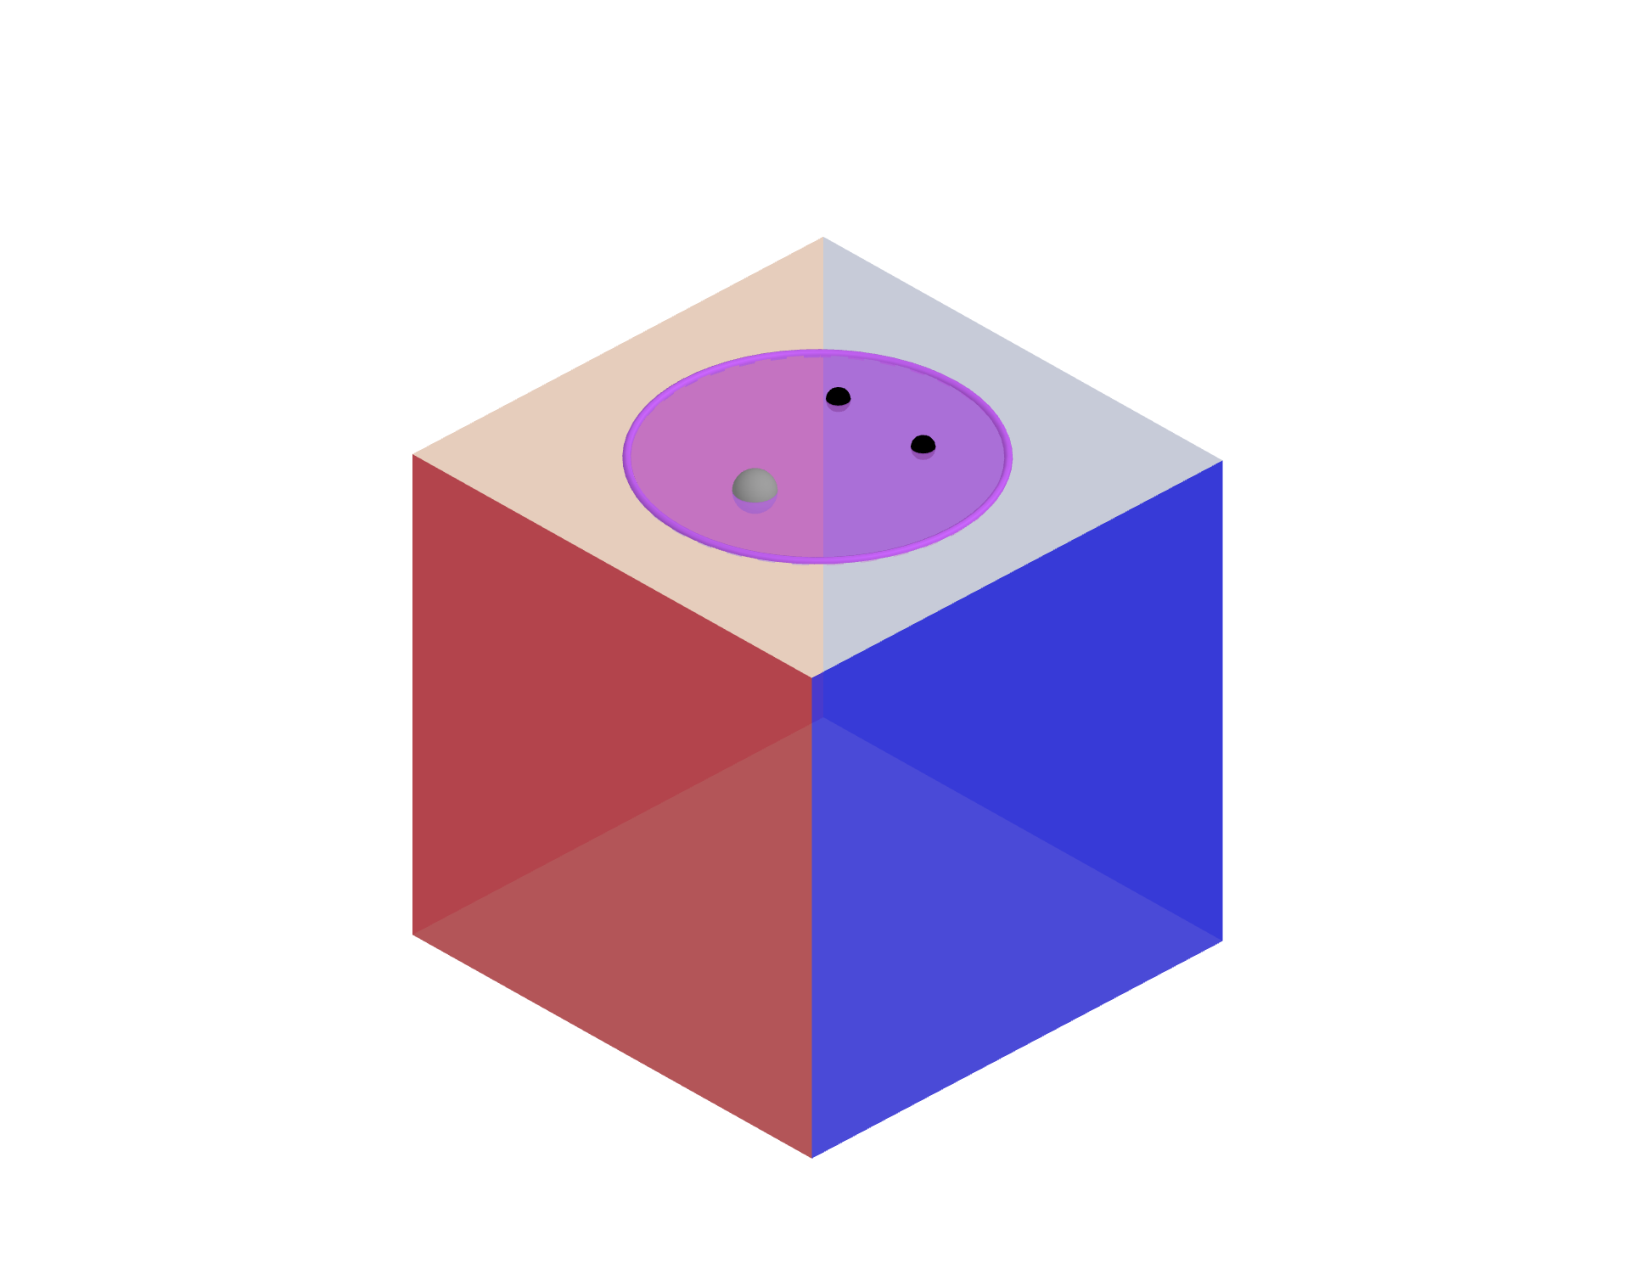
\includegraphics[width=35mm]{figs/curved_cube/curved_cube1of4.pdf}}}\!\!\!\!\!\!\to\!\!\!\!\!\! \)
  \( \vcenter{\hbox{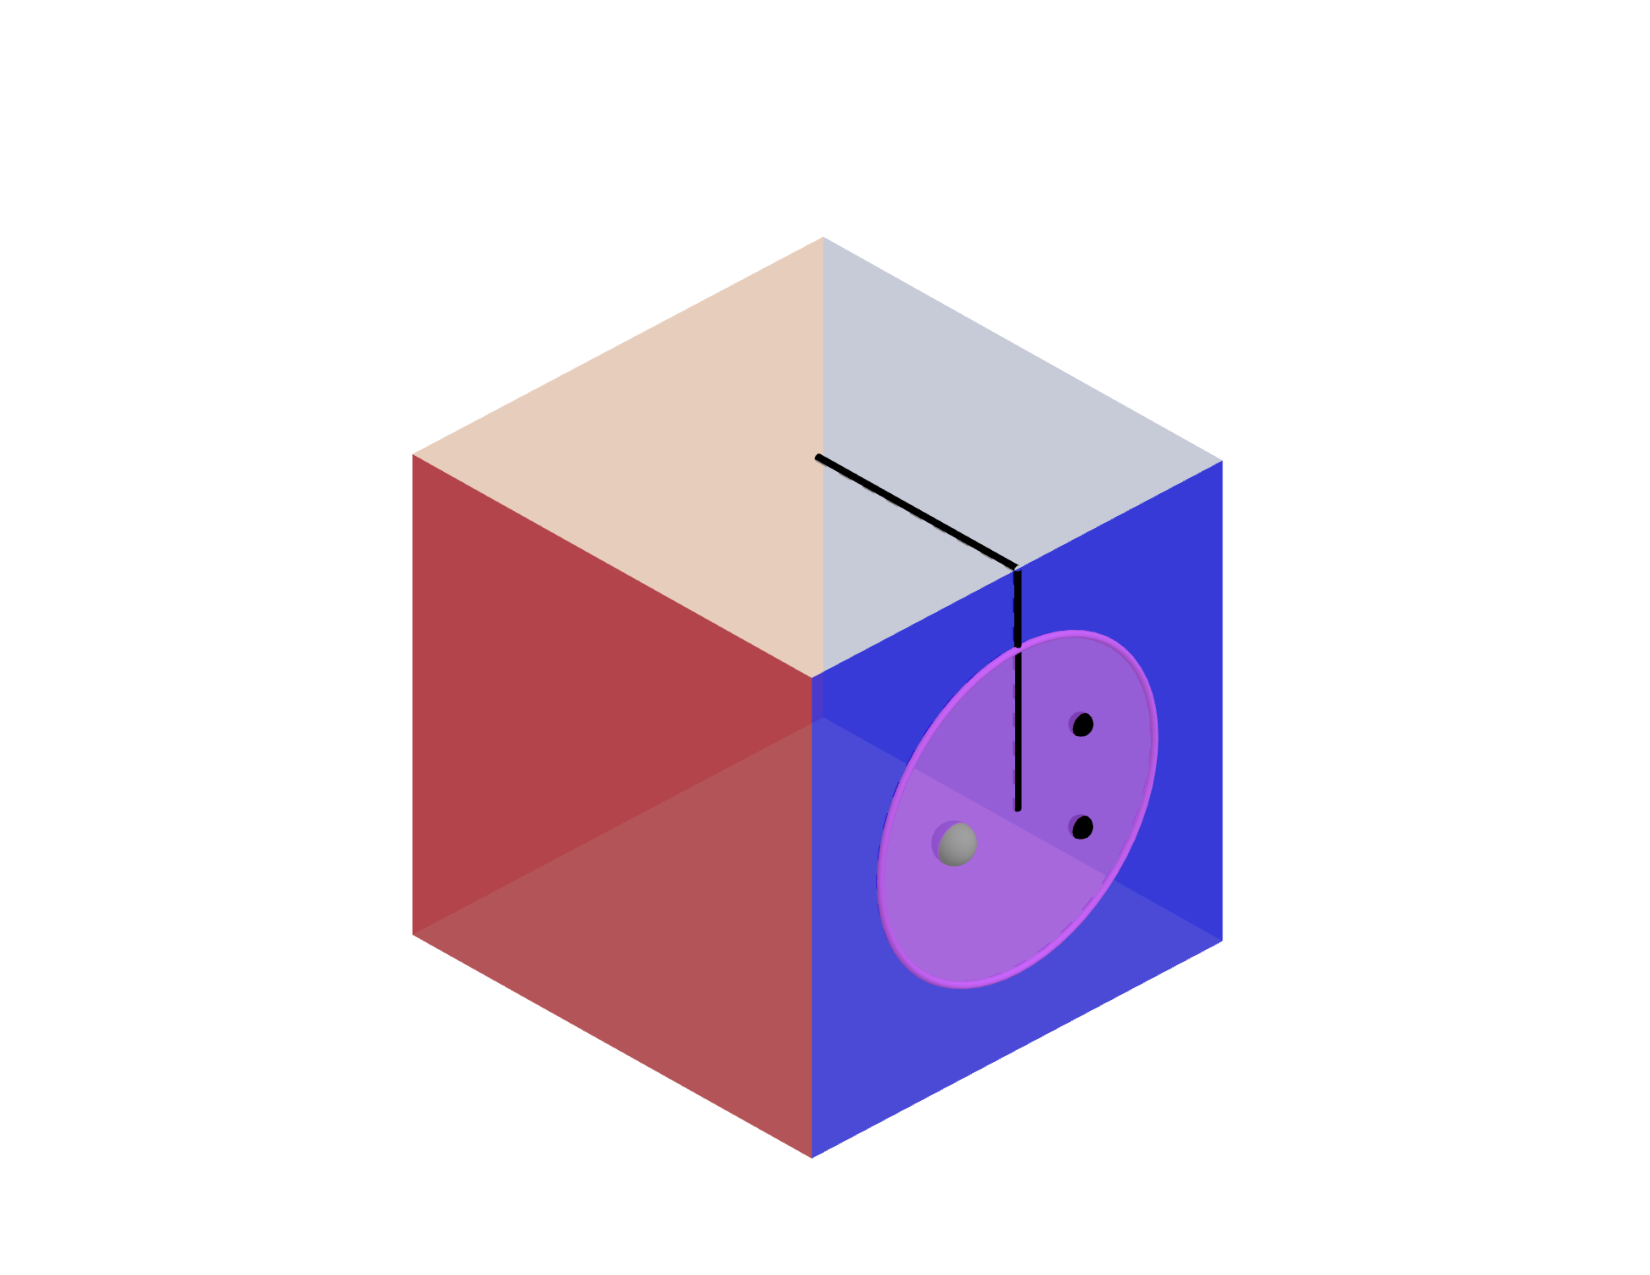
\includegraphics[width=35mm]{figs/curved_cube/curved_cube2of4.pdf}}}\!\!\!\!\!\!\to\!\!\!\!\!\! \)
  \( \vcenter{\hbox{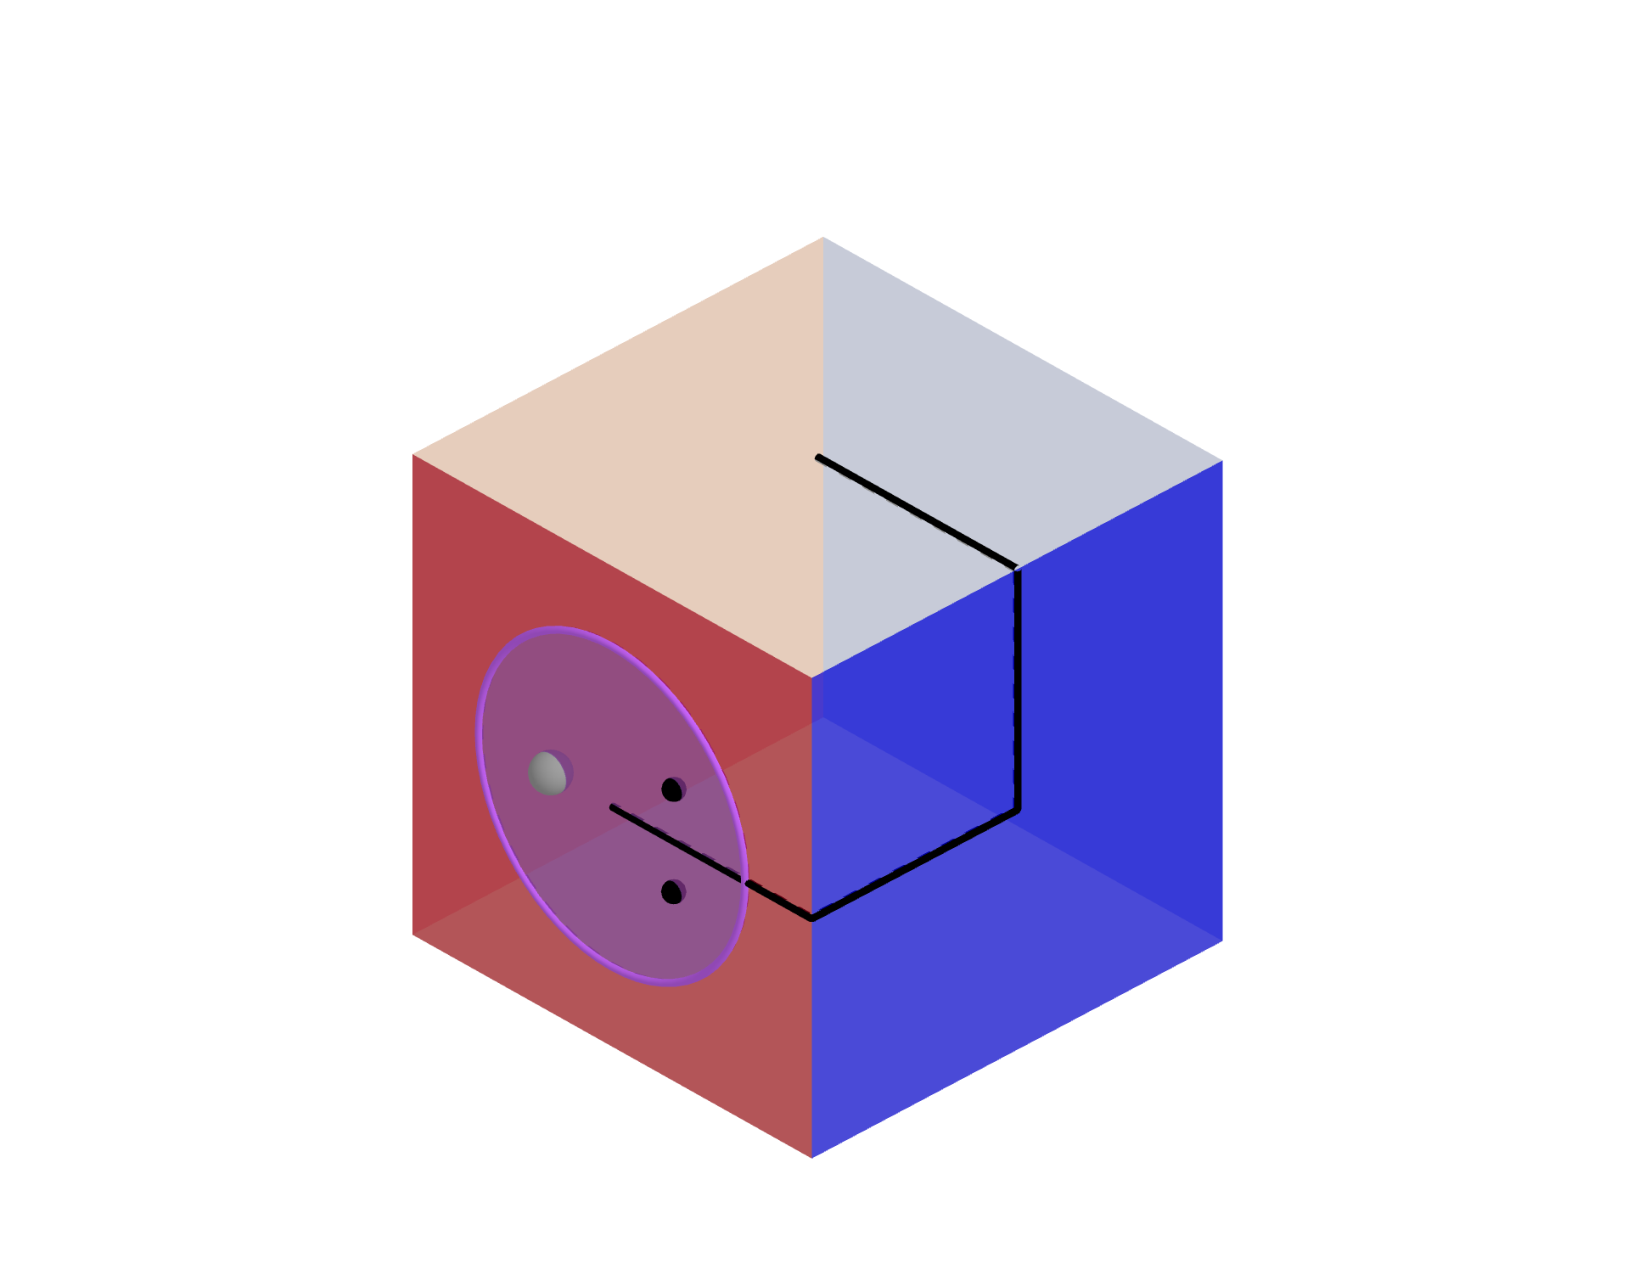
\includegraphics[width=35mm]{figs/curved_cube/curved_cube3of4.pdf}}}\!\!\!\!\!\!\to\!\!\!\!\!\! \)
  \( \vcenter{\hbox{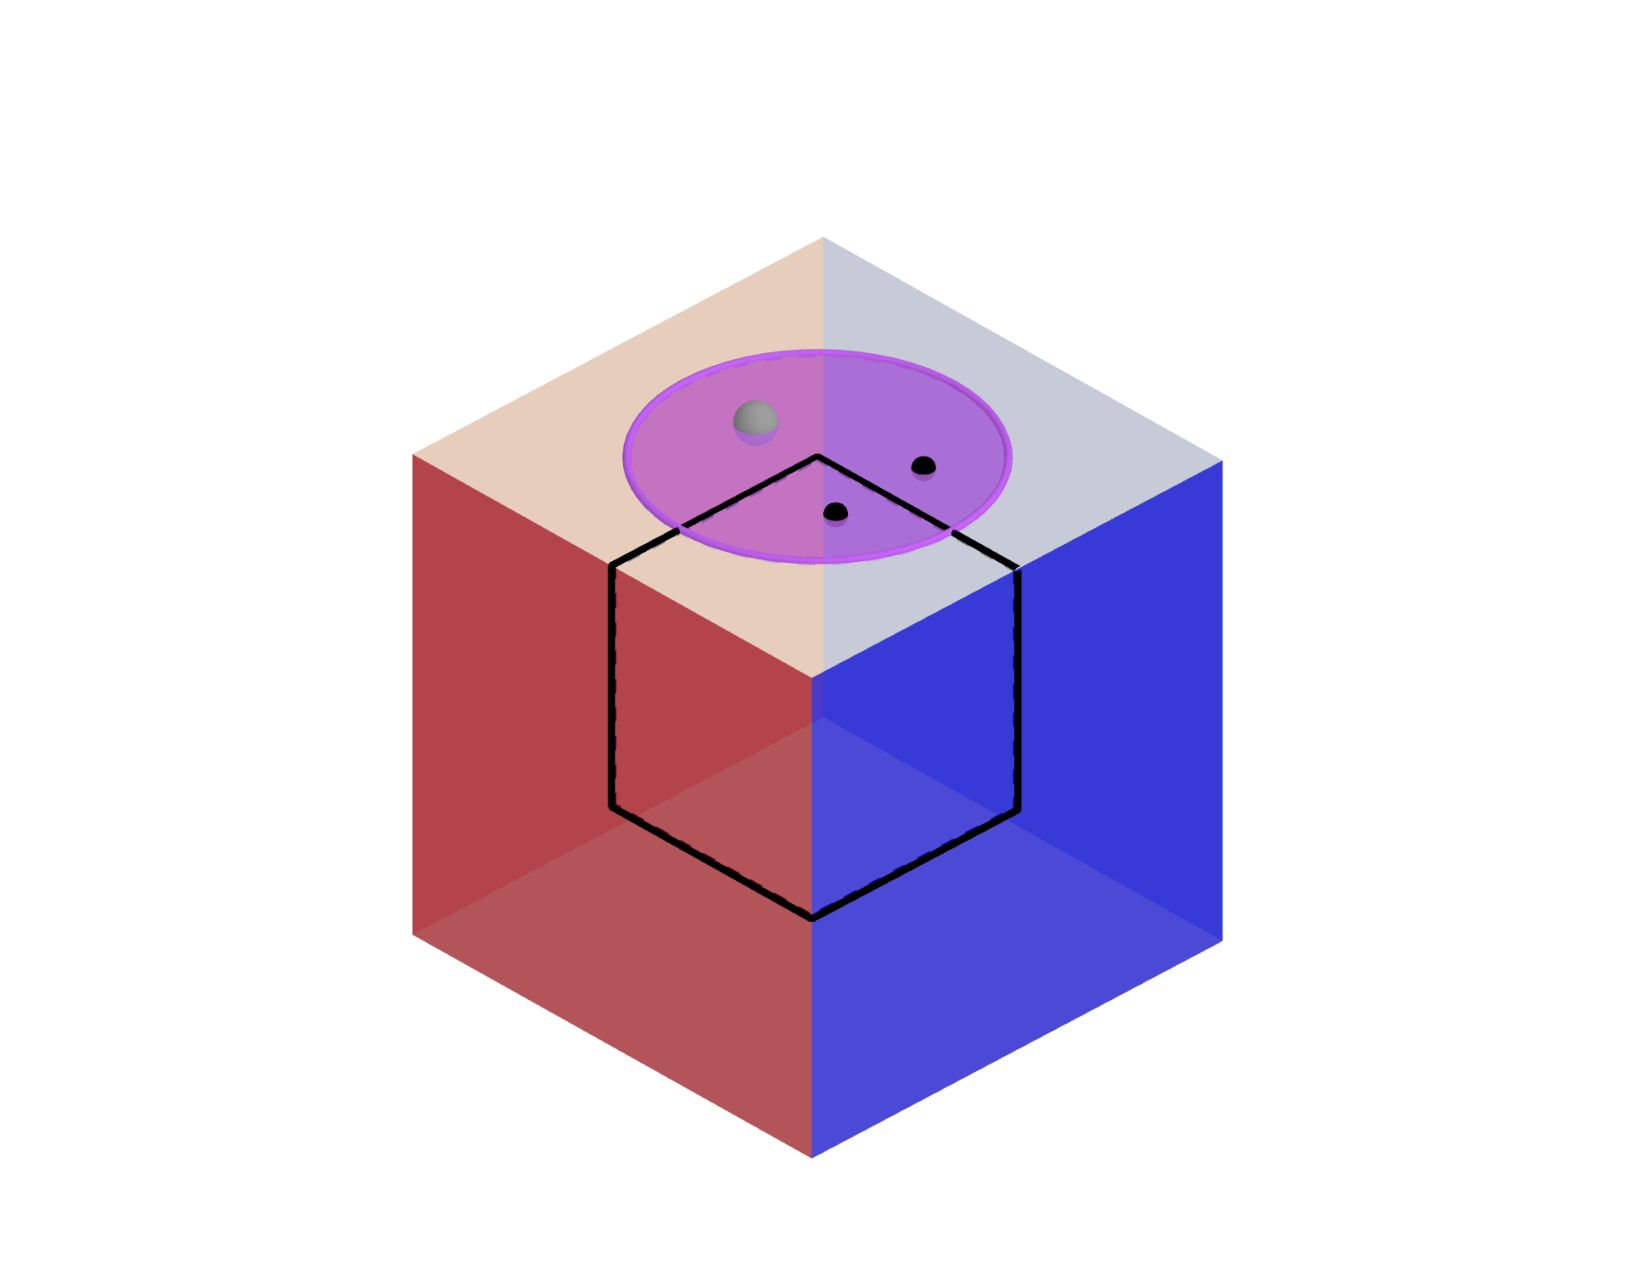
\includegraphics[width=35mm]{figs/curved_cube/curved_cube4of4.pdf}}} \)
\end{frame}

\begin{frame}{The definition of a connection}
\begin{definition}
If \( \mm\defeq \mm_0\xrightarrow[]{\imath_0}\cdots\xrightarrow[]{\imath_{n-1}}\mm_n \) is a combinatorial manifold and all the triangles commute in the diagram:
\[\begin{tikzcd}[ampersand replacement=\&, column sep=small]
  {\mm_0} \& {\mm_1} \& {\mm_2} \& \cdots \& {\mm_n} \\
\&\& {\mathcal{U}}
\arrow["{\imath_0}", from=1-1, to=1-2]
\arrow["{f_0}", from=1-1, to=2-3]
\arrow["{\imath_1}", from=1-2, to=1-3]
\arrow["{f_1}", from=1-2, to=2-3]
\arrow["{\imath_2}", from=1-3, to=1-4]
\arrow["{f_2}", from=1-3, to=2-3]
\arrow["{\imath_{n-1}}", from=1-4, to=1-5]
\arrow["f_n"', from=1-5, to=2-3]
\end{tikzcd}\]
\begin{itemize}
\item The map \( f_k \) is a \defemph{\( k \)-bundle} on \( \mm \).
\item The pair given by the map \( f_k \) and the proof \( f_k\circ \imath_{k-1}=f_{k-1} \), i.e. that \( f_k \) extends \( f_{k-1} \) is called a \defemph{\( k \)-connection on the \( (k-1) \)-bundle \( f_{k-1} \)}.
\end{itemize}
\end{definition}
\end{frame}

\begin{frame}{The definition of curvature}
\begin{mydef}[cont.]
\begin{columns}[t]
\begin{column}{0.55\textwidth}
The pushout consists of \( M_2 \)-many extensions:
\[\begin{tikzcd}[ampersand replacement=\&, column sep=small]
  {M_2\times \partial\Dd(2)} \& {M_2} \\
  {\mathbb{M}_{1}} \& {\mathbb{M}_2} \\
  \& {\mathcal{U}}
  \arrow["{\mathrm{pr}_1}", from=1-1, to=1-2]
  \arrow["{\mathbb{A}_{1}}"', from=1-1, to=2-1]
  \arrow["{}", from=1-2, to=2-2]
  \arrow["{h_2}", shorten <=10pt, shorten >=10pt, Rightarrow, from=2-1, to=1-2]
  \arrow["{}", from=2-1, to=2-2]
  \arrow[""{name=0, anchor=center, inner sep=0}, "{T_{1}}"', from=2-1, to=3-2]
  \arrow["\ulcorner"{pos=-0.05, rotate=180}, shift left=1.5, draw=none, from=2-2, to=1-1]
  \arrow["{T_2}", from=2-2, to=3-2]
  \arrow["{}", shorten >=3pt, Rightarrow, from=2-2, to=0]
\end{tikzcd}\]
\end{column}
\begin{column}{0.45\textwidth}
Here's the outer square for a single face \( F \):
\[\begin{tikzcd}[ampersand replacement=\&]
  {\{F\}\times \partial\Dd(2)} \& \{F\} \\
  {\mathbb{M}_{1}} \& {\mathcal{U}}
  \arrow["{\pr_1}", from=1-1, to=1-2]
  \arrow["{\mathbb{A}_{1}}"', from=1-1, to=2-1]
  \arrow["{}", from=1-2, to=2-2]
  \arrow["{\flat_F}", shorten <=11pt, shorten >=11pt, Rightarrow, from=1-2, to=2-1]
  \arrow[from=2-1, to=2-2]
\end{tikzcd}\]
\end{column}
\end{columns}
\onslide<2->{\( T_1(\partial(F)) \) is \defemph{the curvature at the face \( F \)} and the filler \( \flat_F:\id=T_1(\partial F) \) is called a \defemph{flatness structure for the face \( F \)}.}

\onslide<3->{The distinction between the path \( \flat_F \) and the endpoint \( T_1(\partial(F)) \) is small enough to be confusing.}
\end{mydef}
\end{frame}

% \begin{frame}
% With these definitions we have now achieved one of our main goals.
% 
% On to vector fields.
% \end{frame}


\section{Vector fields}

\begin{frame}{Vector fields}
\begin{columns}
\begin{column}{0.7\textwidth}
Let \( T:\mm\to BS^1 \) be an oriented tangent bundle on a 2-dim combinatorial manifold.
\begin{itemize}
\item Bundles of circles can only model \alert{nonzero} tangent vectors.
\item  A global section would be a trivialization of \( T \), so there is an obstruction.
\end{itemize}
\quad\\~\\
\onslide<2->{
Our solution:
\begin{itemize}
\item<3-> A \alert{vector field} is a term \alert{\( X:\pit{m:\mm_1}Tm \)}.
\item<4-> It's a \alert{nonvanishing} vector field on the 1-skeleton.
\item<5-> We model classical zeros by omitting the faces.
\end{itemize}
}
\end{column}
\begin{column}{0.3\textwidth}
\begin{tikzpicture}%
  [x={(-0.860769cm, -0.121512cm)},
  y={(0.508996cm, -0.205391cm)},
  z={(-0.000053cm, 0.971107cm)},
  scale=1,
  back/.style={loosely dotted, thin},
  edge/.style={black, thick},
  arrow/.style={black, very thick, solid, -{Stealth[scale=0.8]}},
  facet/.style={fill=blue!95!black,fill opacity=0.0},
  vertex/.style={inner sep=1pt,circle,draw=green!25!black,fill=black,thick}]
%% Drawing the vertices in the front
%%
\begin{scope}[nodes=vertex]
\node[label=above right:\( b \)] at (-1, 1, 0) (b)     {};
\node[label=below:\( y \)] at (0, 0, -1.4) (y)    {};
\node[label=above:\( w \)] at (0, 0, 1.4)  (w)   {};
\node[label=above left:\( g \)] at (1, -1, 0) (g)    {};
\node[label=above left:\( r \)] at (1, 1, 0)  (r)   {};
\node[label=above right:\( o \)] at (-1, -1, 0) (o)    {};
\end{scope}
%% Drawing edges in the back
%%
\draw[edge,back,arrow] (o) -- (b);
\draw[edge,back,arrow] (y) -- (o);
\draw[edge,back] (o) -- (w);
\draw[edge,back] (o) -- (g);
%% Drawing vertices in the back
%%
\node[vertex] at (o)     {};
%% Drawing the facets
%%
\fill[facet] (1, 1, 0) -- (0, 0, -1.4) -- (1, -1, 0) -- cycle {};
\fill[facet] (1, 1, 0) -- (0, 0, 1.4) -- (1, -1, 0) -- cycle {};
\fill[facet] (1, 1, 0) -- (-1, 1, 0) -- (0, 0, 1.4) -- cycle {};
\fill[facet] (1, 1, 0) -- (-1, 1, 0) -- (0, 0, -1.4) -- cycle {};
%% Drawing edges in the front
%%
\draw[edge,arrow] (b) -- (y);
\draw[edge] (b) -- (w);
\draw[edge] (b) -- (r);
\draw[edge] (y) -- (g);
\draw[edge] (y) -- (r);
\draw[edge,arrow] (g) -- (w);
\draw[edge,arrow] (w) -- (r);
\draw[edge,arrow] (r) -- (g);
\end{tikzpicture}

\end{column}
\end{columns}
\end{frame}

\begin{frame}{Reminder: pathovers}
\begin{columns}
\begin{column}{0.35\textwidth}
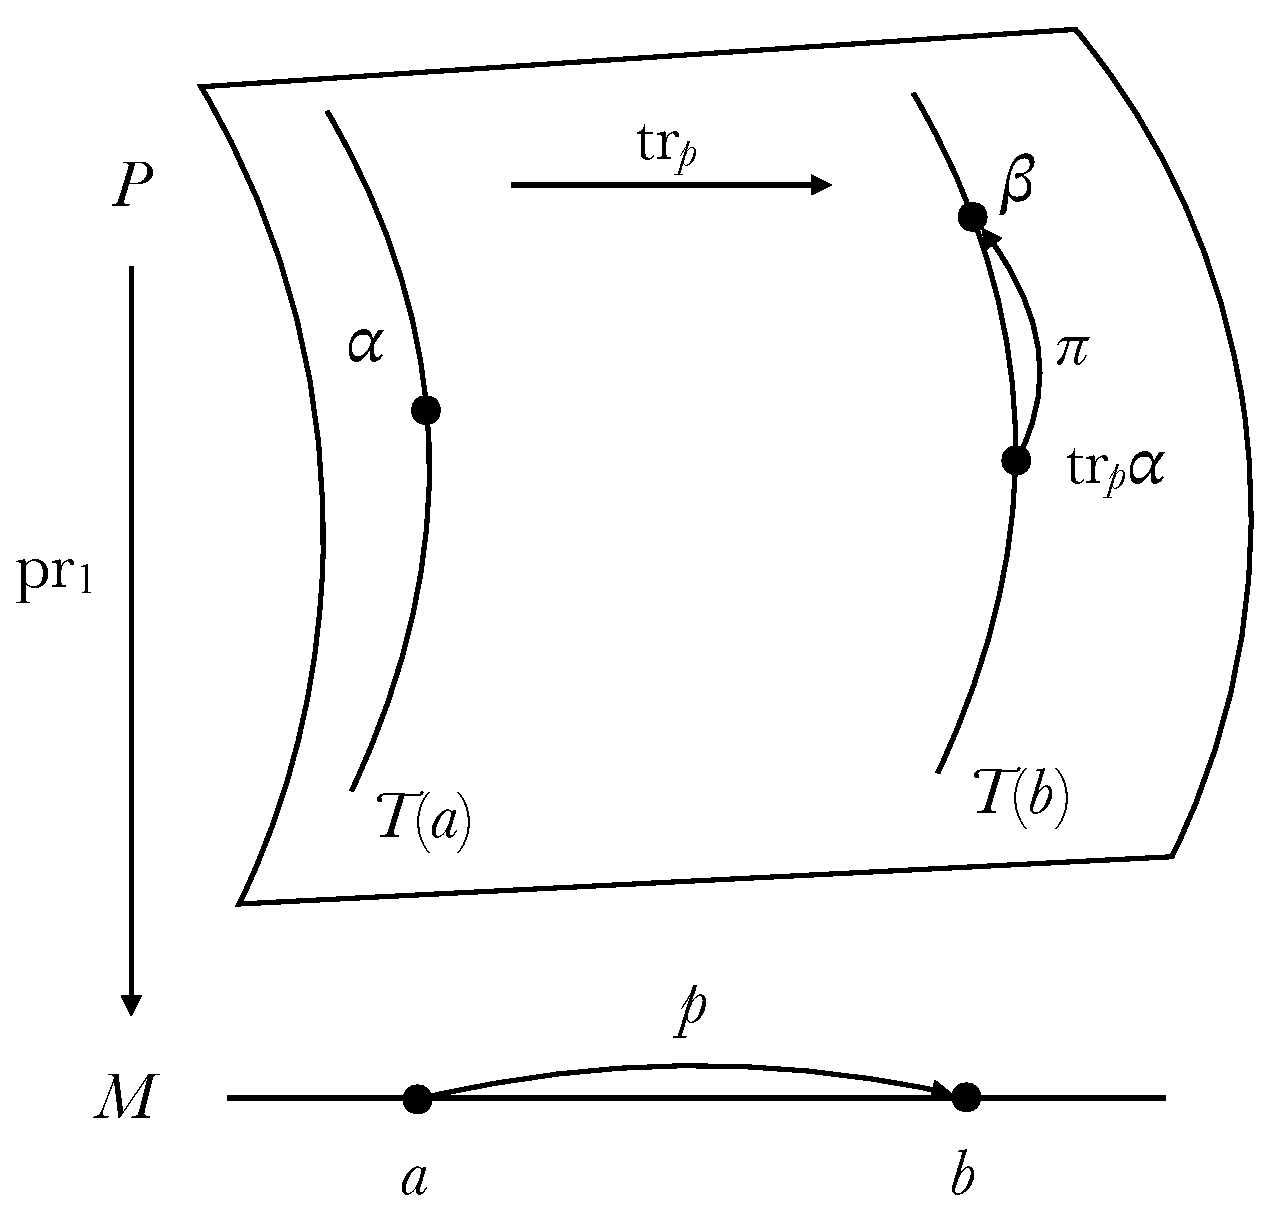
\includegraphics[width=30ex]{figs/pathovers.pdf}
\end{column}
\begin{column}{0.65\textwidth}
\begin{itemize}
\item Recall pathovers (dependent paths).
\item There is an asymmetry: we pick a fiber to display \( \pi \), the path over \( p \).
\item Dependent functions map paths to pathovers: \( \apd (X)(p):\tr_p(X(a))=X(b) \) (simply denoted \( X(p) \)).
\end{itemize}
\end{column}
\end{columns}
\end{frame}

\begin{frame}
Next goal: define the index of a vector field on a face.
\end{frame}

\begin{frame}
\begin{columns}
\begin{column}{0.65\textwidth}
\vspace{12pt}
\begingroup
\tikzset{every picture/.style={scale=0.85}}
\begin{tikzpicture}
  [arrow/.style={-{Stealth[scale=1.1]}}, vec/.style={ultra thick, color=black}, vectr/.style={thick, color=black}, vectrtr/.style={thick, dashed, color=black}, vectrtrtr/.style={thick, dotted, color=black}]
  \tikzset{oo/.style={circle, scale=0.6, fill=black}}
  \tikzset{ii/.style={circle, scale=0.3, fill=gray}}
\newlength{\mylen}
  \setlength{\mylen}{3cm}
  \newlength{\mylin}
  \setlength{\mylin}{0.5cm}
    \node[oo, label=below:\( v_1 \)] (V1) at (0, 0) {};
    \node[oo, label=below:\( v_2 \)] (V2) at (2*\mylen, 0) {};
    \node[oo, label=above:\( v_3 \)] (V3) at (\mylen, 1.732*\mylen) {};

    \draw[arrow] (V2) edge[very thick, color=teal, "\( e_{23} \)"] (V3);
    \draw[arrow] (V1) edge[very thick, color=magenta, "\( e_{12} \)"] (V2);
    \draw[arrow] (V3) edge[very thick, color=blue, "\( e_{31} \)"] (V1);
    
    \node [left=1.3\mylin of  V1,  label=center:\( T_1 \)] {};
    \node [right=1.3\mylin of  V2,  label=center:\( T_2 \)] {};
    \node [left=1.3\mylin of  V3,  label=center:\( T_3 \)] {};

\end{tikzpicture}

\endgroup
\end{column}
\begin{column}{0.35\textwidth}
We will try to show the \alert{three} ingredients of \( X \) on this face:
\begin{itemize}
\item The value of \( X \) on vertices.
\item The value of \( X \) on edges.
\item The transport between vertices, interacting with \( X \).
\end{itemize}
\end{column}
\end{columns}
\end{frame}

\begin{frame}
\begin{columns}
\begin{column}{0.65\textwidth}
\vspace{12pt}
\begingroup
\tikzset{every picture/.style={scale=0.85}}
\begin{tikzpicture}
  [arrow/.style={-{Stealth[scale=1.1]}}, vec/.style={ultra thick, color=black}, vectr/.style={thick, color=black}, vectrtr/.style={thick, dashed, color=black}, vectrtrtr/.style={thick, dotted, color=black}]
  \tikzset{oo/.style={circle, scale=0.6, fill=black}}
  \tikzset{ii/.style={circle, scale=0.3, fill=gray}}
  \setlength{\mylen}{3cm}
  \setlength{\mylin}{1.2cm}
    \node[oo, label=below right:\( v_1 \)] (V1) at (0, 0) {};
    \node[oo, label=below:\( v_3 \)] (V3) at (2*\mylen, 0) {};
    \node[oo, label=above:\( v_2 \)] (V2) at (\mylen, 1.732*\mylen) {};

    \draw[arrow] (V2) edge[very thick, color=teal, "\( e_{23} \)"] (V3);
    \draw[arrow] (V1) edge[very thick, color=magenta, "\( e_{12} \)"] (V2);
    \draw[arrow] (V3) edge[very thick, color=blue, "\( e_{31} \)"] (V1);
    
    \node [ii, above right=\mylin of V1] (V11) {};
    \node [ii, below right=\mylin of V1] (V14) {};
    \node [ii, below left=\mylin of  V1] (V13) {};
    \node [ii, above left= \mylin of V1] (V12) {};

    \node [left=1.3\mylin of  V1,  label=center:\( T_1 \)] {};
    \node [right=1.3\mylin of  V2,  label=center:\( T_2 \)] {};
    \node [right=1.3\mylin of  V3,  label=center:\( T_3 \)] {};

    \node [ii, above right=\mylin of V2] (V21) {};
    \node [ii, below right=\mylin of V2] (V24) {};
    \node [ii, below left=\mylin of  V2] (V23) {};
    \node [ii, above left= \mylin of V2] (V22) {};

    \node [ii, above right=\mylin of V3] (V31) {};
    \node [ii, below right=\mylin of V3] (V34) {};
    \node [ii, below left=\mylin of  V3] (V33) {};
    \node [ii, above left= \mylin of V3] (V32) {};

    \draw[dashed] (V11) -- (V12);
    \draw[dashed] (V12) -- (V13);
    \draw[dashed] (V13) -- (V14);
    \draw[dashed] (V14) -- (V11);

    \draw[dashed] (V21) -- (V22);
    \draw[dashed] (V22) -- (V23);
    \draw[dashed] (V23) -- (V24);
    \draw[dashed] (V24) -- (V21);
    
    \draw[dashed] (V31) -- (V32);
    \draw[dashed] (V32) -- (V33);
    \draw[dashed] (V33) -- (V34);
    \draw[dashed] (V34) -- (V31);
    
    \draw[arrow] (V1) edge[vec] (V11);
\end{tikzpicture}

\endgroup
\end{column}
\begin{column}{0.35\textwidth}
\begin{itemize}
\item<1-> Denote by \( X_1 \) this vector \( X(v_1):T_1 \).
\item<1-> \phantom{Say \( T_{12} \) is trivial. Denote the transported vector as thinner.}
\item<1-> \phantom{Say \( T_{23} \) rotates counterclockwise. Denote the twice-transported vector as dashed.}
\item<1-> \phantom{Say \( T_{31} \) is trivial. The thrice-transported vecor is dotted.}
\end{itemize}
\end{column}
\end{columns}
\end{frame}

\begin{frame}
\begin{columns}
\begin{column}{0.65\textwidth}
\vspace{12pt}
\begingroup
\tikzset{every picture/.style={scale=0.85}}
\begin{tikzpicture}
  [arrow/.style={-{Stealth[scale=1.1]}}, vec/.style={ultra thick, color=black}, vectr/.style={thick, color=black}, vectrtr/.style={thick, dashed, color=black}, vectrtrtr/.style={thick, dotted, color=black}]
  \tikzset{oo/.style={circle, scale=0.6, fill=black}}
  \tikzset{ii/.style={circle, scale=0.3, fill=gray}}
  \setlength{\mylen}{3cm}
  \setlength{\mylin}{1.2cm}
    \node[oo, label=below right:\( v_1 \)] (V1) at (0, 0) {};
    \node[oo, label=below:\( v_2 \)] (V2) at (2*\mylen, 0) {};
    \node[oo, label=above:\( v_3 \)] (V3) at (\mylen, 1.732*\mylen) {};

    \draw[arrow] (V2) edge[very thick, color=teal, "\( e_{23} \)"] (V3);
    \draw[arrow] (V1) edge[very thick, color=magenta, "\( e_{12} \)"] (V2);
    \draw[arrow] (V3) edge[very thick, color=blue, "\( e_{31} \)"] (V1);
    
    \node [ii, above right=\mylin of V1] (V11) {};
    \node [ii, below right=\mylin of V1] (V12) {};
    \node [ii, below left=\mylin of  V1] (V13) {};
    \node [ii, above left= \mylin of V1] (V14) {};

    \node [left=1.3\mylin of  V1,  label=center:\( T_1 \)] {};
    \node [right=1.3\mylin of  V2,  label=center:\( T_2 \)] {};
    \node [left=1.3\mylin of  V3,  label=center:\( T_3 \)] {};

    \node [ii, above right=\mylin of V2] (V21) {};
    \node [ii, below right=\mylin of V2] (V22) {};
    \node [ii, below left=\mylin of  V2] (V23) {};
    \node [ii, above left= \mylin of V2] (V24) {};

    \node [ii, above right=\mylin of V3] (V31) {};
    \node [ii, below right=\mylin of V3] (V32) {};
    \node [ii, below left=\mylin of  V3] (V33) {};
    \node [ii, above left= \mylin of V3] (V34) {};

    \draw[dashed] (V11) -- (V12);
    \draw[dashed] (V12) -- (V13);
    \draw[dashed] (V13) -- (V14);
    \draw[dashed] (V14) -- (V11);

    \draw[dashed] (V21) -- (V22);
    \draw[dashed] (V22) -- (V23);
    \draw[dashed] (V23) -- (V24);
    \draw[dashed] (V24) -- (V21);
    
    \draw[dashed] (V31) -- (V32);
    \draw[dashed] (V32) -- (V33);
    \draw[dashed] (V33) -- (V34);
    \draw[dashed] (V34) -- (V31);
    
    \draw[arrow] (V1) edge[vec] (V11);
    \draw[arrow] (V2) edge[vectr] (V21);
\end{tikzpicture}

\endgroup
\end{column}
\begin{column}{0.35\textwidth}
\begin{itemize}
\item<1-> Denote by \( X_1 \) this vector \( X(v_1):T_1 \).
\item<1-> Say \( T_{12} \) is trivial. Denote the transported vector as thinner.
\item<1-> \phantom{Say \( T_{23} \) rotates counterclockwise. Denote the twice-transported vector as dashed.}
\item<1-> \phantom{Say \( T_{31} \) is trivial. The thrice-transported vecor is dotted.}
\end{itemize}
\end{column}
\end{columns}
\end{frame}

\begin{frame}
\begin{columns}
\begin{column}{0.65\textwidth}
\vspace{12pt}
\begingroup
\tikzset{every picture/.style={scale=0.85}}
\begin{tikzpicture}
  [arrow/.style={-{Stealth[scale=1.1]}}, vec/.style={ultra thick, color=black}, vectr/.style={thick, color=black}, vectrtr/.style={thick, dashed, color=black}, vectrtrtr/.style={thick, dotted, color=black}]
  \tikzset{oo/.style={circle, scale=0.6, fill=black}}
  \tikzset{ii/.style={circle, scale=0.3, fill=gray}}
  \setlength{\mylen}{3cm}
  \setlength{\mylin}{1.2cm}
    \node[oo, label=below right:\( v_1 \)] (V1) at (0, 0) {};
    \node[oo, label=below:\( v_3 \)] (V3) at (2*\mylen, 0) {};
    \node[oo, label=above:\( v_2 \)] (V2) at (\mylen, 1.732*\mylen) {};

    \draw[arrow] (V2) edge[very thick, color=teal, "\( e_{23} \)"] (V3);
    \draw[arrow] (V1) edge[very thick, color=magenta, "\( e_{12} \)"] (V2);
    \draw[arrow] (V3) edge[very thick, color=blue, "\( e_{31} \)"] (V1);
    
    \node [ii, above right=\mylin of V1] (V11) {};
    \node [ii, below right=\mylin of V1] (V14) {};
    \node [ii, below left=\mylin of  V1] (V13) {};
    \node [ii, above left= \mylin of V1] (V12) {};

    \node [left=1.3\mylin of  V1,  label=center:\( T_1 \)] {};
    \node [right=1.3\mylin of  V2,  label=center:\( T_2 \)] {};
    \node [right=1.3\mylin of  V3,  label=center:\( T_3 \)] {};

    \node [ii, above right=\mylin of V2] (V21) {};
    \node [ii, below right=\mylin of V2] (V24) {};
    \node [ii, below left=\mylin of  V2] (V23) {};
    \node [ii, above left= \mylin of V2] (V22) {};

    \node [ii, above right=\mylin of V3] (V31) {};
    \node [ii, below right=\mylin of V3] (V34) {};
    \node [ii, below left=\mylin of  V3] (V33) {};
    \node [ii, above left= \mylin of V3] (V32) {};

    \draw[dashed] (V11) -- (V12);
    \draw[dashed] (V12) -- (V13);
    \draw[dashed] (V13) -- (V14);
    \draw[dashed] (V14) -- (V11);

    \draw[dashed] (V21) -- (V22);
    \draw[dashed] (V22) -- (V23);
    \draw[dashed] (V23) -- (V24);
    \draw[dashed] (V24) -- (V21);
    
    \draw[dashed] (V31) -- (V32);
    \draw[dashed] (V32) -- (V33);
    \draw[dashed] (V33) -- (V34);
    \draw[dashed] (V34) -- (V31);
    
    \draw[arrow] (V1) edge[vec] (V11);
    \draw[arrow] (V2) edge[vectr] (V21);
    \draw[arrow] (V3) edge[vectrtr] (V34);
\end{tikzpicture}

\endgroup
\end{column}
\begin{column}{0.35\textwidth}
\begin{itemize}
\item<1-> Denote by \( X_1 \) this vector \( X(v_1):T_1 \).
\item<1-> Say \( T_{12} \) is trivial. Denote the transported vector as thinner.
\item<1-> Say \( T_{23} \) rotates counterclockwise. Denote the twice-transported vector as dashed.
\item<1-> \phantom{Say \( T_{31} \) is trivial. The thrice-transported vecor is dotted.}
\end{itemize}
\end{column}
\end{columns}
\end{frame}

\begin{frame}
\begin{columns}
\begin{column}{0.65\textwidth}
\vspace{12pt}
\begingroup
\tikzset{every picture/.style={scale=0.85}}
\begin{tikzpicture}
  [arrow/.style={-{Stealth[scale=1.1]}}, vec/.style={ultra thick, color=black}, vectr/.style={thick, color=black}, vectrtr/.style={thick, dashed, color=black}, vectrtrtr/.style={thick, dotted, color=black}]
  \tikzset{oo/.style={circle, scale=0.6, fill=black}}
  \tikzset{ii/.style={circle, scale=0.3, fill=gray}}
  \setlength{\mylen}{3cm}
  \setlength{\mylin}{1.2cm}
    \node[oo, label=below right:\( v_1 \)] (V1) at (0, 0) {};
    \node[oo, label=below:\( v_3 \)] (V3) at (2*\mylen, 0) {};
    \node[oo, label=above:\( v_2 \)] (V2) at (\mylen, 1.732*\mylen) {};

    \draw[arrow] (V2) edge[very thick, color=teal, "\( e_{23} \)"] (V3);
    \draw[arrow] (V1) edge[very thick, color=magenta, "\( e_{12} \)"] (V2);
    \draw[arrow] (V3) edge[very thick, color=blue, "\( e_{31} \)"] (V1);
    
    \node [ii, above right=\mylin of V1] (V11) {};
    \node [ii, below right=\mylin of V1] (V14) {};
    \node [ii, below left=\mylin of  V1] (V13) {};
    \node [ii, above left= \mylin of V1] (V12) {};

    \node [left=1.3\mylin of  V1,  label=center:\( T_1 \)] {};
    \node [right=1.3\mylin of  V2,  label=center:\( T_2 \)] {};
    \node [right=1.3\mylin of  V3,  label=center:\( T_3 \)] {};

    \node [ii, above right=\mylin of V2] (V21) {};
    \node [ii, below right=\mylin of V2] (V24) {};
    \node [ii, below left=\mylin of  V2] (V23) {};
    \node [ii, above left= \mylin of V2] (V22) {};

    \node [ii, above right=\mylin of V3] (V31) {};
    \node [ii, below right=\mylin of V3] (V34) {};
    \node [ii, below left=\mylin of  V3] (V33) {};
    \node [ii, above left= \mylin of V3] (V32) {};

    \draw[dashed] (V11) -- (V12);
    \draw[dashed] (V12) -- (V13);
    \draw[dashed] (V13) -- (V14);
    \draw[dashed] (V14) -- (V11);

    \draw[dashed] (V21) -- (V22);
    \draw[dashed] (V22) -- (V23);
    \draw[dashed] (V23) -- (V24);
    \draw[dashed] (V24) -- (V21);
    
    \draw[dashed] (V31) -- (V32);
    \draw[dashed] (V32) -- (V33);
    \draw[dashed] (V33) -- (V34);
    \draw[dashed] (V34) -- (V31);
    
    \draw[arrow] (V1) edge[vec] (V11);
    \draw[arrow] (V2) edge[vectr] (V21);
    \draw[arrow] (V3) edge[vectrtr] (V34);
    \draw[arrow] (V1) edge[vectrtrtr] (V14);

\end{tikzpicture}

\endgroup
\end{column}
\begin{column}{0.35\textwidth}
\begin{itemize}
\item<1-> Denote by \( X_1 \) this vector \( X(v_1):T_1 \).
\item<1-> Say \( T_{12} \) is trivial. Denote the transported vector as thinner.
\item<1-> Say \( T_{23} \) rotates counterclockwise. Denote the twice-transported vector as dashed.
\item<1-> Say \( T_{31} \) is trivial. The thrice-transported vecor is dotted.
\end{itemize}
\end{column}
\end{columns}
\end{frame}

\begin{frame}
\begin{columns}
\begin{column}{0.65\textwidth}
\vspace{12pt}
\begingroup
\tikzset{every picture/.style={scale=0.85}}
\begin{tikzpicture}
  [arrow/.style={-{Stealth[scale=1.1]}}, vec/.style={ultra thick, color=black}, vectr/.style={thick, color=black}, vectrtr/.style={thick, dashed, color=black}, vectrtrtr/.style={thick, dotted, color=black}]
  \tikzset{oo/.style={circle, scale=0.6, fill=black}}
  \tikzset{ii/.style={circle, scale=0.3, fill=gray}}
  \setlength{\mylen}{3cm}
  \setlength{\mylin}{1.2cm}
    \node[oo, label=below right:\( v_1 \)] (V1) at (0, 0) {};
    \node[oo, label=below:\( v_3 \)] (V3) at (2*\mylen, 0) {};
    \node[oo, label=above:\( v_2 \)] (V2) at (\mylen, 1.732*\mylen) {};

    \draw[arrow] (V2) edge[very thick, color=teal, "\( e_{23} \)"] (V3);
    \draw[arrow] (V1) edge[very thick, color=magenta, "\( e_{12} \)"] (V2);
    \draw[arrow] (V3) edge[very thick, color=blue, "\( e_{31} \)"] (V1);
    
    \node [ii, above right=\mylin of V1] (V11) {};
    \node [ii, below right=\mylin of V1] (V14) {};
    \node [ii, below left=\mylin of  V1] (V13) {};
    \node [ii, above left= \mylin of V1] (V12) {};

    \node [left=1.3\mylin of  V1,  label=center:\( T_1 \)] {};
    \node [right=1.3\mylin of  V2,  label=center:\( T_2 \)] {};
    \node [right=1.3\mylin of  V3,  label=center:\( T_3 \)] {};

    \node [ii, above right=\mylin of V2] (V21) {};
    \node [ii, below right=\mylin of V2] (V24) {};
    \node [ii, below left=\mylin of  V2] (V23) {};
    \node [ii, above left= \mylin of V2] (V22) {};

    \node [ii, above right=\mylin of V3] (V31) {};
    \node [ii, below right=\mylin of V3] (V34) {};
    \node [ii, below left=\mylin of  V3] (V33) {};
    \node [ii, above left= \mylin of V3] (V32) {};

    \draw[dashed] (V11) -- (V12);
    \draw[dashed] (V12) -- (V13);
    \draw[dashed] (V13) -- (V14);
    \draw[dashed] (V14) -- (V11);

    \draw[dashed] (V21) -- (V22);
    \draw[dashed] (V22) -- (V23);
    \draw[dashed] (V23) -- (V24);
    \draw[dashed] (V24) -- (V21);
    
    \draw[dashed] (V31) -- (V32);
    \draw[dashed] (V32) -- (V33);
    \draw[dashed] (V33) -- (V34);
    \draw[dashed] (V34) -- (V31);
    
    \draw[arrow] (V1) edge[vec] (V11);
    \draw[arrow] (V2) edge[vectr] (V21);
    \draw[arrow] (V3) edge[vectrtr] (V34);
    \draw[arrow] (V1) edge[vectrtrtr] (V14);

    \draw[arrow] (V2) edge[vec] (V24);
    \draw[arrow] (V3) edge[vectr] (V33);
    \draw[arrow] (V1) edge[vectrtr] (V13);

    \draw[arrow] (V21) edge[thick, color=magenta] (V24);
    \draw[arrow] (V34) edge[thick, color=magenta] (V33);
    \draw[arrow] (V14) edge[thick, color=magenta] (V13);
    \draw[arrow] (V33) edge[thick, color=teal] (V32);
    \draw[arrow] (V13) edge[thick, color=teal] (V12);
    \draw[arrow] (V12) edge[thick, color=blue] (V11);

    \draw[arrow] (V3) edge[vec] (V32);
    \draw[arrow] (V1) edge[vectr] (V12);
\end{tikzpicture}

\endgroup
\end{column}
\begin{column}{0.35\textwidth}
\begin{itemize}
\item<1-> \( X \) on \( e_{12} \) is red, etc.
\item<2-> We translated all results to the end of the loop.
\item<3-> (Reminds me of scooping ice cream towards the last fiber.)
\end{itemize}
\end{column}
\end{columns}
\end{frame}

\begin{frame}{Symbolic version}
\begin{tikzcd}[ampersand replacement=\&, row sep=small]
  {T_1} \& {T_2} \& {T_3} \& {T_1} \\
  \&\&\& {T_{13}T_{32}T_{21}X_1} \\
  \&\& {T_{32}T_{21}X_1} \& {T_{13}T_{32}X_2} \\
  \& {T_{21}X_1} \& {T_{32}X_2} \& {T_{13}X_3} \\
  {X_1} \& {X_2} \& {X_3} \& {X_1}
  \arrow["{T_{21}}", from=1-1, to=1-2]
  \arrow["{T_{32}}", from=1-2, to=1-3]
  \arrow["{T_{13}}", from=1-3, to=1-4]
  \arrow["{\alert{T_{13}T_{32}X_{12}}:}", equals, from=3-4, to=2-4]
  \arrow["{\alert{X_{12}}:}"', equals, from=4-2, to=5-2]
  \arrow["{\alert{T_{32}X_{12}}:}", equals, from=4-3, to=3-3]
  \arrow["{\alert{T_{13}X_{23}}:}", equals, from=4-4, to=3-4]
  \arrow["{\alert{X_{23}}:}", equals, from=5-3, to=4-3]
  \arrow["{\alert{X_{31}}:}", equals, from=5-4, to=4-4]
\end{tikzcd}
\end{frame}

\begin{frame}{Index}
\[\begin{aligned}
\tr_F&\defeq \tr(\partial F)&&:T_1=_{BS^1}T_1&&\text{\alert{curvature}}\\
\flat_F&\defeq \flat(\partial F)&&:\id=_{(T_1=_{BS^1}T_1)}\tr_F&&\text{\alert{flatness}}\\
X_F&\defeq X(\partial F)&&:\tr_F(X_1)=_{T_1}X_1&&\text{\alert{swirling}}\\
\end{aligned}\]
\onslide<2->{Recall that \( T_1 \) being an \( S^1 \)-torsor means we can use subtraction to obtain an equivalence \( s(-,X_1):T_1\xrightarrow[]{x\mapsto x\alert{-X_1}} S^1 \).
\begin{columns}[c]
\begin{column}{0.7\textwidth}
\begin{mydef}
The \defemph{flattened swirling} of the vector field \( X \) on the face \( F \) is the loop \[ L^X_F\defeq\flat_F(X_1)\cdot X_F:(X_1=_{T_1}X_1). \]

The \defemph{index} of the vector field \( X \) on the face \( F \) is the integer \( I^X_F \) such that \( \loopo^{I^X_F}=_{S^1}(L^X_F)-X_1 \).
\end{mydef}
\end{column}
\begin{column}{0.3\textwidth}
\begin{tikzpicture}
  [arrow/.style={-{Stealth[scale=1.1]}}, .style={scale=0.7}, vec/.style={ultra thick, color=black}, vectr/.style={thick, color=black}, vectrtr/.style={thick, dashed, color=black}, vectrtrtr/.style={thick, dotted, color=black}]
  \tikzset{oo/.style={circle, scale=0.6, fill=black}}
  \tikzset{ii/.style={circle, scale=0.3, fill=gray}}
  \setlength{\mylen}{2cm}
  \setlength{\mylin}{1cm}
  %\node[label=center:\( Tv_1 \)] (V1) at (0, 0) {};
  \node [ii, above right=\mylin of V1] (V11) {};
  \node [ii, below right=\mylin of V1] (V12) {};
  \node [ii, below left=\mylin of  V1] (V13) {};
  \node [ii, above left= \mylin of V1] (V14) {};
  \node[oo, label=right:\( v_1 \)] (V1) at (0, 0) {};

  \draw[dashed] (V11) edge[ultra thick, solid, arrow, swap, "\( \flat_F(X_1) \)"] (V14);
  \draw[arrow] (V14) edge[thick, swap, color=magenta, "\( X_{12} \)"] (V13);
  \draw[arrow] (V13) edge[thick, swap, color=teal, "\( X_{23} \)"] (V12);
  \draw[arrow] (V12) edge[thick, swap, color=blue, "\( X_{31} \)"] (V11);
  \draw[arrow] (V1) edge[vec] (V11);
    \draw[arrow] (V1) edge[vectrtrtr] (V14);
    \draw[arrow] (V1) edge[vectrtr] (V13);
    \draw[arrow] (V1) edge[vectr] (V12);
\end{tikzpicture}
\end{column}
\end{columns}}
\end{frame}


\section{Main theorem}
\newcommand{\Xij}{X_{ij}}
\newcommand{\Xji}{X_{ji}}
\newcommand{\Tij}{T_{ij}}
\newcommand{\Tji}{T_{ji}}
\newcommand{\sij}{\sigma_{ij}}
\newcommand{\sji}{\sigma_{ji}}
\newcommand{\rij}{\rho_{ij}}
\newcommand{\rji}{\rho_{ji}}
\newcommand{\dotcirc}{\odot}

\begin{frame}{Simplifying swirling}
Swirling involves concatenating dependent paths. Can we simplify that?
\end{frame}

\begin{frame}{Pay off all our assumptions 1: torsor structure, vector field}
\begin{columns}
\begin{column}{0.15\textwidth}
\begin{tikzcd}[ampersand replacement=\&, column sep=small]
  {T_1} \\
  {T_{13}T_{32}T_{21}X_1} \\
  {T_{13}T_{32}X_2} \\
  {T_{13}X_3} \\
  {X_1}
  \arrow["{\alert{T_{13}T_{32}X_{21}}:}", equals, from=3-1, to=2-1]
  \arrow["{\alert{T_{13}X_{32}}:}", equals, from=4-1, to=3-1]
  \arrow["{\alert{X_{13}}:}", equals, from=5-1, to=4-1]
\end{tikzcd}

\end{column}
\begin{column}{0.85\textwidth}
\begin{itemize}
\item<2-> Def: \( \alpha_i\defeq s(-,X_i):T_i\simto S^1 \) (\alert{trivialization on 0-skeleton}).
\item<3-> Def: \( \rji\defeq \alpha_j(\Tji(X_i)) \) is \alert{the rotation of \( \Tji \)}.
% https://q.uiver.app/#q=WzAsNCxbMCwwLCJUX2kiXSxbMSwwLCJUX2oiXSxbMCwxLCJTXjEiXSxbMSwxLCJTXjEiXSxbMCwxLCJUX3tqaX0iXSxbMCwyLCJcXGFscGhhX2kiLDJdLFsxLDMsIlxcYWxwaGFfaiJdLFsyLDMsIigtKVxcY2RvdFxccmhvX3tqaX0iLDJdLFszLDEsIlxcbWF0aHNme2Jhc2V9XFxtYXBzdG8gWF9qIiwyLHsib2Zmc2V0IjozLCJjdXJ2ZSI6MX1dLFsyLDAsIlxcbWF0aHNme2Jhc2V9XFxtYXBzdG8gWF9pIiwwLHsib2Zmc2V0IjotMywiY3VydmUiOi0xfV1d
\[\begin{tikzcd}[ampersand replacement=\&]
  {T_i} \& {T_j} \\
  {S^1} \& {S^1}
  \arrow["{T_{ji}}", from=1-1, to=1-2]
  \arrow["{\alpha_i}"', from=1-1, to=2-1]
  \arrow["{\alpha_j}", from=1-2, to=2-2]
  \arrow["{\mathsf{base}\mapsto X_i}", shift left=3, curve={height=-6pt}, from=2-1, to=1-1]
  \arrow["{(-)\dotcirc\rho_{ji}}"', from=2-1, to=2-2]
  \arrow["{\mathsf{base}\mapsto X_j}"', shift right=3, curve={height=6pt}, from=2-2, to=1-2]
\end{tikzcd}\]
\item<4-> Lemma: \( \rij=\rji^{-1} \) because \alert{in \( T_j \)}: \( \rij\dotcirc\rji\dotcirc X_j=\rij\dotcirc \Tji X_i=\Tji(\rij\dotcirc X_i)=\Tji \Tij X_j=X_j \).
\end{itemize}
\end{column}
\end{columns}
\end{frame}

\begin{frame}{Pay off all our assumptions 1: torsor structure, vector field (cont.)}
\begin{columns}
\begin{column}{0.15\textwidth}
\begin{tikzcd}[ampersand replacement=\&, column sep=small]
  {T_1} \\
  {T_{13}T_{32}T_{21}X_1} \\
  {T_{13}T_{32}X_2} \\
  {T_{13}X_3} \\
  {X_1}
  \arrow["{\alert{T_{13}T_{32}X_{21}}:}", equals, from=3-1, to=2-1]
  \arrow["{\alert{T_{13}X_{32}}:}", equals, from=4-1, to=3-1]
  \arrow["{\alert{X_{13}}:}", equals, from=5-1, to=4-1]
\end{tikzcd}

\end{column}
\begin{column}{0.85\textwidth}
\begin{itemize}
\item<2-> Define \( \sji\defeq \alpha_j(\Xji):\rji=_{S^1}\base, \).
\item<3-> Paths of the form \( (a=_{S^1}\base) \) can be multiplied: 
\begin{itemize}
\item \( \dotcirc:(a=\base)\times (b=base)\to (a\dotcirc b=base) \).
\item \( p\dotcirc q=(p\dotcirc b)\cdot q. \)
\end{itemize}
\item<4-> Lemma: \( \apd(X)(\refl)=\refl\) \(\implies \Xij\cdot \Tij\Xji=\refl_{X_i}\) \(\implies\sij\dotcirc\sji=\refl_{\base} \) (\( \Tij \) just translates \( \Xji \) to cat with \( \Xji \)).
\end{itemize}
\end{column}
\end{columns}
\end{frame}

\begin{frame}{Pay off all our assumptions 2: no boundary, commutativity}
\begin{columns}
\begin{column}{0.15\textwidth}
\begin{tikzcd}[ampersand replacement=\&, column sep=small]
  {T_1} \\
  {T_{13}T_{32}T_{21}X_1} \\
  {T_{13}T_{32}X_2} \\
  {T_{13}X_3} \\
  {X_1}
  \arrow["{\alert{T_{13}T_{32}X_{21}}:}", equals, from=3-1, to=2-1]
  \arrow["{\alert{T_{13}X_{32}}:}", equals, from=4-1, to=3-1]
  \arrow["{\alert{X_{13}}:}", equals, from=5-1, to=4-1]
\end{tikzcd}

\end{column}
\begin{column}{0.85\textwidth}
\begin{mydef}
Let \( F_1,\ldots,F_n \) be the faces of \( \mm \), and \( \partial F_1,\ldots,\partial F_n \) be the triangular boundaries. The \alert{total swirling} is \[ X_\tot \defeq \sigma_{\partial F_1}\dotcirc\cdots\dotcirc\sigma_{\partial F_n} \].
\end{mydef}
\begin{itemize}
\item<2-> We assume that this expression involves \alert{every edge once in each direction}.
\item<3-> \( S^1 \) is commutative, hence \alert{complete cancellation}.
\end{itemize}
\end{column}
\end{columns}
\end{frame}


\begin{frame}{Consequence}
\[\begin{aligned}
\tr_F&\defeq \tr(\partial F)&&:T_1=_{BS^1}T_1&&\text{\alert{curvature}}\\
\flat_F&\defeq \flat(\partial F)&&:\id=_{(T_1=_{BS^1}T_1)}\tr_F&&\text{\alert{flatness}}\\
X_F&\defeq X(\partial F)&&:\tr_F(X_1)=_{T_1}X_1&&\text{\alert{swirling}}\\
L^X_F&\defeq\flat_F(X_1)\cdot X_F&&:(X_1=_{T_1}X_1)&&\text{\alert{flattened swirling}}
\end{aligned}\]
\onslide<2->{
These can all be totaled in \( S^1 \) to give
\begin{columns}[t]
\begin{column}{0.5\textwidth}
\[\begin{aligned}
\tr_\tot&\defeq \bigodot_i \rho_{\partial F} = \base\\
\flat_\tot&\defeq \bigodot_i\flat_{\partial F}\\
\end{aligned}\]
\end{column}
\begin{column}{0.5\textwidth}
\[\begin{aligned}
X_\tot&\defeq \bigodot_i \sigma_{\partial F} = \refl_\base\\
L^X_\tot&\defeq \bigodot_i \flat_{\partial F} \dotcirc \sigma_{\partial F} = \bigodot_i \flat_{\partial F}
\end{aligned}\]
\end{column}
\end{columns}
}\onslide<3->{
So in our lingo: the total flatness equals the total flattened swirling.\qed
}
\end{frame}

\begin{frame}{Classical proof}
\begin{columns}
\column{0.5\textwidth}
\vspace{12pt}
\begin{figure}
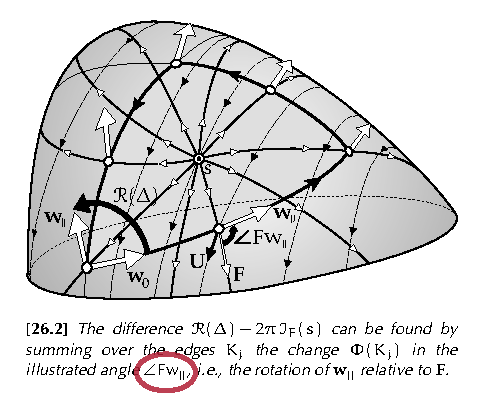
\includegraphics[width=0.9\textwidth]{figs/needham_triangle_circ.pdf}
\caption{{Needham,~T. (2021) Visual Differential Geometry and Forms.}}
\end{figure}
\column{0.5\textwidth}
\vspace{-12pt}
\begin{itemize}
\item The classical proof is discrete-flavored.
\item ``\( \angle Fw_{||} \)'' looked a lot like a pathover.
\item Hopf's \( \Phi \) is defined on edges, not loops. We imitated that too.
\end{itemize}
\end{columns}
\end{frame}



\begin{frame}
\begin{center}
\alert{\huge{Thank you!}}
\end{center}
\end{frame}

\section{Appendix}
\begin{frame}{Dictionary}
\begin{tabular}{|p{18em}|p{18em}|}
\hline
Connections are 1-forms on \( P \) not on \( M \) & \( T(e_{ij}):T_i=T_j \), which is not a loop. \\ \hline
Space of connections for a given \( P \) is contractible. & \\ \hline
Euler class & \\ \hline
\end{tabular}
\end{frame}

\begin{frame}{Dictionary}
\begin{tabular}{|p{18em}|p{18em}|}
\hline
Poincare dual & \\ \hline
Leibniz rule & \\ \hline
Transport is not infinitesimal & \\ \hline
\end{tabular}
\end{frame}

\begin{frame}{Dictionary}
\begin{tabular}{|p{18em}|p{18em}|}
\hline
State a thm like: if \( w_1, w_2 \) and \( c_1 \) are equal on \( P_1, P_2 \) then \( P_1=P_2 \) & \\ \hline
Is cohomology about the type of maps, and \( F \) gives a term? & \\ \hline
Hopf fibration should give another map \( \oo_2\to\EMzo \). & \\ \hline
\end{tabular}
\end{frame}

\begin{frame}{Dictionary}
\begin{tabular}{|p{18em}|p{18em}|}
\hline
Maurer-Cartan form. & \\ \hline
Gauge transformations acting on connections and maybe functions (YM) of connections. & \\ \hline
The based gauge group acts freely on connections. & \\ \hline
\end{tabular}
\end{frame}
\end{document}



